%%%%%%%%%%%%%%%%%%%%%%%%%%%%%%%%%%%%%%%%%
% McMaster Masters/Doctoral Thesis
% LaTeX Template
% Version 2.2 (11/23/15)
%
% This template has been downloaded from:
% http://www.LaTeXTemplates.com
% Then subsequently from http://www.overleaf.com
%
% Version 2.0 major modifications by:
% Vel (vel@latextemplates.com)
%
% Original authors:
% Steven Gunn  (http://users.ecs.soton.ac.uk/srg/softwaretools/document/templates/)
% Sunil Patel (http://www.sunilpatel.co.uk/thesis-template/)
%
% Modified to McMaster format by Benjamin Furman (contact: https://www.xenben/com; Most up
% to date template at https://github.com/benjaminfurman/McMaster_Thesis_Template,
% occasionally updated on Overleaf template page)
%
% Modified for macdown by Antonio Paez; most up to date version at https://github.com/paezha/macdown
%
% License:
% CC BY-NC-SA 3.0 (http://creativecommons.org/licenses/by-nc-sa/3.0/)
%
%%%%%%%%%%%%%%%%%%%%%%%%%%%%%%%%%%%%%%%%%

%----------------------------------------------------------------------------------------
% DOCUMENT CONFIGURATIONS
%----------------------------------------------------------------------------------------

\documentclass[
11pt, % The default document font size, options: 10pt, 11pt, 12pt
oneside, % Two side (alternating margins) for binding by default, uncomment to switch to one side
english, % other languages available
singlespacing, % Single line spacing, alternatives: onehalfspacing or doublespacing
%draft, % Uncomment to enable draft mode (no pictures, no links, overfull hboxes indicated)
%nolistspacing, % If the document is onehalfspacing or doublespacing, uncomment this to set spacing in lists to single
%liststotoc, % Uncomment to add the list of figures/tables/etc to the table of contents
%toctotoc, % Uncomment to add the main table of contents to the table of contents
]{macthesis} % The class file specifying the document structure

%----------------------------------------------------------------------------------------
% Import packages here
%----------------------------------------------------------------------------------------
\usepackage[utf8]{inputenc} % Required for inputting international characters
\usepackage[T1]{fontenc} % Output font encoding for international characters
\usepackage{lastpage} % count pages
\usepackage{lmodern} % could change font type by calling a different package
\usepackage{lscape} % for landscaping pages
% New commands for landscape orientation
\newcommand{\blandscape}{\begin{landscape}}
\newcommand{\elandscape}{\end{landscape}}
%
\usepackage{siunitx} % for scientific units (micro-liter, etc)
\setcounter{tocdepth}{2} % so that only section and sub sections appear in Table of Contents. Remove or set depth to 3 to include sub-sub-sections

%----------------------------------------------------------------------------------------
% Define a blank page
%----------------------------------------------------------------------------------------
\def\blankpage{%
      \clearpage%
      \thispagestyle{empty}%
      \addtocounter{page}{-1}%
      \null%
      \clearpage}

%----------------------------------------------------------------------------------------
% Define a tight list
%----------------------------------------------------------------------------------------
\def\tightlist{}

%----------------------------------------------------------------------------------------
%	Highlight Code Chunks
%----------------------------------------------------------------------------------------

%----------------------------------------------------------------------------------------
% Handling Citations
%----------------------------------------------------------------------------------------

% definitions for citeproc citations
\NewDocumentCommand\citeproctext{}{}
\NewDocumentCommand\citeproc{mm}{%
\begingroup\def\citeproctext{#2}\cite{#1}\endgroup}
\makeatletter
% allow citations to break across lines
\let\@cite@ofmt\@firstofone
% avoid brackets around text for \cite:
\def\@biblabel#1{}
\def\@cite#1#2{{#1\if@tempswa , #2\fi}}
\makeatother
\newlength{\cslhangindent}
\setlength{\cslhangindent}{1.5em}
\newlength{\csllabelwidth}
\setlength{\csllabelwidth}{3em}
\newenvironment{CSLReferences}[2] % #1 hanging-indent, #2 entry-spacing
{\begin{list}{}{%
	\setlength{\itemindent}{0pt}
	\setlength{\leftmargin}{0pt}
	\setlength{\parsep}{0pt}
	% turn on hanging indent if param 1 is 1
	\ifodd #1
	\setlength{\leftmargin}{\cslhangindent}
	\setlength{\itemindent}{-1\cslhangindent}
	\fi
	% set entry spacing
	\setlength{\itemsep}{#2\baselineskip}}}
{\end{list}}
\usepackage{calc}
\newcommand{\CSLBlock}[1]{\hfill\break\parbox[t]{\linewidth}{\strut\ignorespaces#1\strut}}
\newcommand{\CSLLeftMargin}[1]{\parbox[t]{\csllabelwidth}{\strut#1\strut}}
\newcommand{\CSLRightInline}[1]{\parbox[t]{\linewidth - \csllabelwidth}{\strut#1\strut}}
\newcommand{\CSLIndent}[1]{\hspace{\cslhangindent}#1}


%----------------------------------------------------------------------------------------
% Collect all your header information from the chapters here, things like acronyms, custom commands, necessary packages, etc.
%----------------------------------------------------------------------------------------
\usepackage{parskip} %this will put spaces between paragraphs
\setlength{\parindent}{15pt} % this will create and indent on all but the first paragraph of each section.
% should maybe change to glossaries package
\usepackage{acro}
\DeclareAcronym{est}{
	short = EST,
	long  = expressed sequence tags
}

\DeclareAcronym{Xl}{
	short = \textit{X.~laevis},
	long  = \textit{Xenopus~laevis}
}
\DeclareAcronym{Xg}{
	short = \textit{X.~gilli},
	long  = \textit{Xenopus~gilli}
}

\usepackage{etoolbox}
\preto\chapter{\acresetall} % resets acronyms for each chapter

\usepackage{xspace} %helps spacing with custom commands.
\newcommand{\oddname}{{\sc SoME goOfY LonG ThiNg With an AwkWarD NAme}\xspace}


\usepackage{pgfplotstable} % a much better way to handle tables
\pgfplotsset{compat=1.12}

% \usepackage{float} % if you need to demand figure/table placement, then this will allow you to use [H], which demands a figure placement. Beware, making LaTeX do things it doesn't want may lead to oddities.


%%%%
% LINK COLORS
% You can control the link colors at the end of the McMasterThesis.cls file. There is also a true/false option there to turn off all link colors.
%%%%


%----------------------------------------------------------------------------------------
%	THESIS INFORMATION
%----------------------------------------------------------------------------------------

\title{A family of accessibility measures: bringing practical interpretation to access inequities}
%\thesistitle{Thesis Title} % Your thesis title, print it elsewhere with \ttitle
\author{Anastasia Soukhov}
%\author{John \textsc{Smith}} % Your name, print it elsewhere with \authorname
\bdegree{B.Eng.}
\mdegree{M.A.Sc.}
%Previous degrees % print it elsewhere with \bdeg and \mdeg
\date{June 2025}
% The month and year that you submit your FINAL draft TO THE LIBRARY (May or December)
\university{McMaster University}
%\university{\href{http://www.mcmaster.ca/}{McMaster University}} % Your university's name and URL, print it elsewhere with \univname
%\division{}
\faculty{Faculty of Science} % Your faculty's name and URL, print it elsewhere with \facname
\department{School of Earth, Environment and Society} % Your department's name and URL, print it elsewhere with \deptname
\subject{Geography} % Your subject area, print it elsewhere with \subjectname
%\group{\href{http://researchgroup.university.com}{Research Group Name}} % Your research group's name and URL, print it elsewhere with \groupname
\supervisor{Antonio Paez}
%\supervisor{Dr. Jane \textsc{Smith}} % Your supervisor's name, print it elsewhere with \supname
\examiner{} % Your examiner's name, print it elsewhere with \examname
\degree{Doctor of Philosophy}
%\degree{Doctor of Philosophy} % Your degree name, print it elsewhere with \degreename
\addresses{} % Your address, print it elsewhere with \addressname
\keywords{} % Keywords for your thesis, print it elsewhere with \keywordnames


% this sets up hyperlinks
\hypersetup{pdftitle=\ttitle} % Set the PDF's title to your title
\hypersetup{pdfauthor=\authorname} % Set the PDF's author to your name
\hypersetup{pdfkeywords=\keywordnames} % Set the PDF's keywords to your keywords

\begin{document}
\sloppy

\frontmatter % Use roman page numbering style (i, ii, iii, iv...) for the pre-content pages

\pagestyle{plain} % Default to the plain heading style until the thesis style is called for the body content

%----------------------------------------------------------------------------------------
%	Half Title (lay title)
%----------------------------------------------------------------------------------------
%\begin{halftitle} % could not get this environment working
%\vspace*{\fill}
\vspace{6cm}
\begin{center}
\ttitle
\end{center}
%\vspace*{\fill}
\pagenumbering{gobble} % leave this here, McMaster doesn't want this page numbered
%\end{halftitle}
\clearpage

%----------------------------------------------------------------------------------------
%	TITLE PAGE
%----------------------------------------------------------------------------------------
\pagenumbering{gobble}
\begin{center}

\vfill
\textsc{\Large \ttitle} \\

\vfill
{By \authorname\, \bdeg \, \mdeg }


 \vfill
{\large \textit{A Thesis Submitted to the School of Graduate Studies in the Partial Fulfillment of the Requirements for the Degree \degreename}}\\

\vfill
{\large \univname\, \copyright\, Copyright by \authorname\, \today}\\[4cm] % replace \today with the submission date

\end{center}
\blankpage
\clearpage

%----------------------------------------------------------------------------------------
%	QUOTATION PAGE
%----------------------------------------------------------------------------------------

\vspace*{0.2\textheight}

\noindent{\itshape SOME QUOTE}\bigbreak

\hfill\textemdash Some author of a quote

\blankpage
\clearpage

%%%%%%%%%%%%%%%%%%%%%%%%%%%
%%%%%%%%%%%%%%%%%%%%%%%%%%%
% optional page stuff
%----------------------------------------------------------------------------------------
% can do physical constraints and symbols pages, see the original thesis example on overleaf if you want to include them at https://www.overleaf.com/latex/templates/template-for-a-masters-slash-doctoral-thesis/mkzrzktcbzfl#.VlPeicorpE4
%----------------------------------------------------------------------------------------

%----------------------------------------------------------------------------------------
%	DEDICATION
%----------------------------------------------------------------------------------------

    You can have a dedication here if you wish.

\blankpage
\clearpage


%----------------------------------------------------------------------------------------
%	Descriptive note numbered ii
%----------------------------------------------------------------------------------------
% Need to add below info
\newpage
\pagenumbering{roman} % leave to turn numbering back on
\setcounter{page}{2} % leave here to make this page numbered ii, a Grad School requirement

\noindent % stops indent on next line
\univname \\
\degreename\, (\the\year) \\
Hamilton, Ontario (\deptname) \\[1.5cm]
TITLE: \ttitle \\
AUTHOR: \authorname\,  %list previous degrees
(\univname)  \\
SUPERVISOR: \supname\, \\
NUMBER OF PAGES: \pageref{lastoffront}, \pageref{LastPage}  % put in iv and number

\clearpage

%----------------------------------------------------------------------------------------
%	Lay abstract number iii
%----------------------------------------------------------------------------------------
% not actually included in most theses, though requested by the GSA
% uncomment below lines if you want to include one
\section*{Lay Abstract}
  (150 words or less).

  The aim of transportation systems is to connect people and opportunities (i.e., jobs, services). However, traditionally transportation planning has focused on mobility (distances travelled), instead of accessibility (how many opportunities can be reached). Experts have been calling for a shift from mobility-based methods to access-based ones, but this change hasn't fully happened yet for a variety of reasons. One challenge is methodological: the lack of clear units for measuring accessibility. This thesis aims to help address this gap by outlining how accessibility methods relate to dominant mobility-based techniques, and how the concept of `constraints' can be borrowed from these techniques to re/introduce units for accessibility measures.
\blankpage
\clearpage


%----------------------------------------------------------------------------------------
%	ABSTRACT PAGE number iv
%----------------------------------------------------------------------------------------

\section*{\Huge Abstract}
\addchaptertocentry{\abstractname}
% Type your abstract here.
Transportation systems plays a fundamental role in cities by facilitating access between people and various social and economic opportunities. Access, otherwise known as Accessibility, can be defined as the potential to spatially interact with opportunities. However, for decades transportation planning has relied on mobility-based estimates and indicators, oriented based on realized movement (e.g., kilometres travelled, emissions released) as opposed to potential movement (e.g., the number of opportunities that can be reached). In recent years, there has been calls to move from mobility-based methods to access-based ones, but a few barriers remain. One signficant issue is methodological, namely, the lack in clarity in the interpretion of conventional accessiblity measures' scores. An emerging approach is to link these scores to outcomes, but this thesis proposes a preceeding step: clarifying the units of accessibility.

In this line, the aim of this thesis is fourfold: 1) review how accessibility literature largely diverged from the spatial interaction literature, but how the addition of a proportionally constaint that both returns the units to the measure and balances them to reflect known constraints in the system may be of use. 2) formally introduce the total constraint, equivalent to the conventional accessibility measure in magnitude but now results are in units of opportunities. 3) introduce the single constraint which considers population competition for opportunities and could be understood as the 2SFCA before normalizing by capita. 4) demonstrate these constrained accessibility measures use on an empirical example of accessibility to parks in Toronto, and how constrained accessibility (i.e.., in units of opportunities) can be used to communicate for the purpose of policy.
\blankpage
\clearpage

%----------------------------------------------------------------------------------------
%	ACKNOWLEDGEMENTS
%----------------------------------------------------------------------------------------

  \begin{acknowledgements}
  \addchaptertocentry{\acknowledgementname} % Add the acknowledgments to the table of contents
    I want to thank a few people. Antonio Paez. Moataz Mohamed. Chris Higgins. Core team. Rafael Perriera. Accessibility nerds at the City of Toronto: dedicated to developing equity thinking in a systematic and rigourous way, Lorina, Michael, Bryce, Herman, and many others.

    Along the way, the mobilizing justice team: Nacho, Matthew Palm, Steven Farber, Joao, Robert. UGs at UpfT and McMaster. Colleagues at McMaster - especially Lea Ravensenberg, that led me to supervise Nicholas Mooney, my first supervisee as a PhD, and an incredible opporuntity to work with Angel and Isla. To colleagues at UPM. Javier, Julio, Carlos. Lab mates Alberto, Manu, Amor, Raul, Manuel and others at TRANSyT. To Colleages at UoFT especially Madealine. And my many friends along the way at the many international conferences, NARSC, AAG, TRB, WCTRS, and especially NECTAR\ldots{}
  \end{acknowledgements}
\blankpage
\clearpage

%----------------------------------------------------------------------------------------
%	LIST OF CONTENTS/FIGURES/TABLES PAGES
%----------------------------------------------------------------------------------------

\tableofcontents % Prints the main table of contents

\listoffigures % Prints the list of figures

\listoftables % Prints the list of tables

%----------------------------------------------------------------------------------------
%	ABBREVIATIONS
%----------------------------------------------------------------------------------------
% many theses don't use this section, as it will be declared at first use and again each chapter. Uncomment these four lines to activate if you want
%\clearpage
%\section*{\Huge Acronyms}
%\addchaptertocentry{Acronyms}
%\printacronyms[name] % name without an option stops the header

%----------------------------------------------------------------------------------------
%	DECLARATION PAGE
%----------------------------------------------------------------------------------------

\begin{declaration}
\addchaptertocentry{\authorshipname}

\noindent I, \authorname, declare that this thesis titled, \emph{\ttitle} and the work presented in it are my own. I confirm that:

I did most of the research.

Also the writing.

Sometimes I cried.

But mostly I had fun.

\end{declaration}


%----------------------------------------------------------------------------------------
% The following bit is just here to make sure we end up on a new page and get the total number of roman numeral
\label{lastoffront}
\clearpage
% make sure this command is on the last of your frontmatter pages, i.e. only this command, a \clearpage then \mainmatter
% should be fine without modification
%----------------------------------------------------------------------------------------

%----------------------------------------------------------------------------------------
%	THESIS MAIN BODY
%----------------------------------------------------------------------------------------

\mainmatter % here the regular arabic numbering starts
\pagestyle{thesis}
\chapter{This is the degree you are aiming for with this thesis}\label{this-is-the-degree-you-are-aiming-for-with-this-thesis}

Placeholder

\section{This dissertation's evolution}\label{this-dissertations-evolution}

\section{The importance of accessibility; and conceptual issues interpreting `unconstrained' access}\label{the-importance-of-accessibility-and-conceptual-issues-interpreting-unconstrained-access}

\section{Aims}\label{aims}

\section{A practical case study: Toronto and publically owned and opertated green space}\label{a-practical-case-study-toronto-and-publically-owned-and-opertated-green-space}

\section{Overview of methods}\label{overview-of-methods}

\subsection{Accessibility metrics}\label{accessibility-metrics}

\subsection{Data sources and travel time estimates}\label{data-sources-and-travel-time-estimates}

\section{Chapters outline}\label{chapters-outline}

\chapter{CHP 1 - A family of accessibility measures}\label{chp-1---a-family-of-accessibility-measures}

THIS CHAPTER IS COPY-PASTE OF THE FORECOMING PAPER \emph{``Family of accessibility measures derived from spatial interaction principles''}

\chapter{CHP 2 - Totally constrained spatial access to park space}\label{chp-2---totally-constrained-spatial-access-to-park-space}

\begin{verbatim}
Linking to GEOS 3.12.2, GDAL 3.9.3, PROJ 9.4.1; sf_use_s2() is TRUE
\end{verbatim}

\begin{verbatim}

Attaching package: 'dplyr'
\end{verbatim}

\begin{verbatim}
The following objects are masked from 'package:stats':

    filter, lag
\end{verbatim}

\begin{verbatim}
The following objects are masked from 'package:base':

    intersect, setdiff, setequal, union
\end{verbatim}

\section{Introduction}\label{introduction}

Urban greenspace has many benefits for residents and the environment: it is linked to wellbeing {[}{]}, higher rates of physical activity {[}{]}, and contributes to reducing urban island heating as well as mitigating carbon pollution in combating climate change {[}{]}. Parkland, or greenspace that is owned and operated by a locality, can also be framed as a public service. In this way, the spatial accessibility to parkland should be concerned with ensuring it is distributed in an equitable way.

In this chapter, the empirical example of parkland city of Toronto will be detailed, including (1) the spatial resolution of the zoning system and the residing population, (2) the assumptions associated with calculating parkland entrance points, and the (3) assumed interaction with parkland. (4) Following the data, the totally-constrained accessibility measure is briefly summarised. The calculated results are presented and interpreted in a policy-relevant lens: namely, the amount of parkland that is accessible per zone, identification of zones with low and high accessibility.

Notably, this process of methods, data and results presentation was done in consultation with staff from the City of Toronto. They are actively working on developing the Transportation Equity Policy Framework and are partners of the Mobilizing Justice Partnership. All data is openly available, but is edited by the city staff (as attributed) or using assumptions the city staff were agreement with.

\section{Methods and Data}\label{methods-and-data}

\subsection{Origins: the dissemination block and associated census data}\label{origins-the-dissemination-block-and-associated-census-data}

The most disaggregated level that census variables (e.g., household income, proportion commute mode) is available is the level of the dissemination area (DA). Census zoning systems are designed by Statistics Canada to represent the population's socioeconomic characteristics as homogeneously, with disaggregated systems (like the DA) requiring to nest within more aggregated systems while remaining a relatively compact geographic size (Statistics Canada, 2021a). Each DA in the Toronto metropolitan area represents population between 441 (Q1) to 836(Q3)) and each representing between 0.0732 sq km (Q1) to 0.2322 sq km (Q3)) in area.

However, population data is available at an even more disaggregated level, the dissemination blocks (DB). The DB is an artifact of the road network (Statistics Canada, 2021b), with between 2 to 5 DBs being typically nested within one DA . The more accurately the origin point represents the known residing population, the more accurately the routed travel time and hence the accessibility results along with its associated assumptions, can be understood. Moreover, the highest level of spatial disaggregation available, is typically the preferred appropriate: to reduce issues associated with the scale effect of the modifiable areal unit problem (MAUP) {[}{]}.

For these reasons, points that are representative of the population within each DB was calculated using the methodology described by Statistics Canada (Statistics Canada, 2021c). These representative points are available through Statistics Canada at the DA level, however, DB level points are not. hence, the calculated DB points, or the DB weighted centroids, were generated by the staff at the City of Toronto, and sent to the author on May 2, 2025. The methodology to prepare the points is summarised as follows: (1) if the DB contained no address points, then the geometric centroid of the DB was used, (2) if the DB contains 1 or more address points, then the central point between the dwelling weighted address points was calculated. If this point was not with the DB boundaries, it was manually moved into the DB.

To contextualise the Toronto metropolitan area, the population (per DB) and the associated DA boundaries plus the cities that compose the Toronto metropolitan area are visualised in Figure \ref{fig:chp2-toronto_CMA_plot}.

\begin{figure}

{\centering 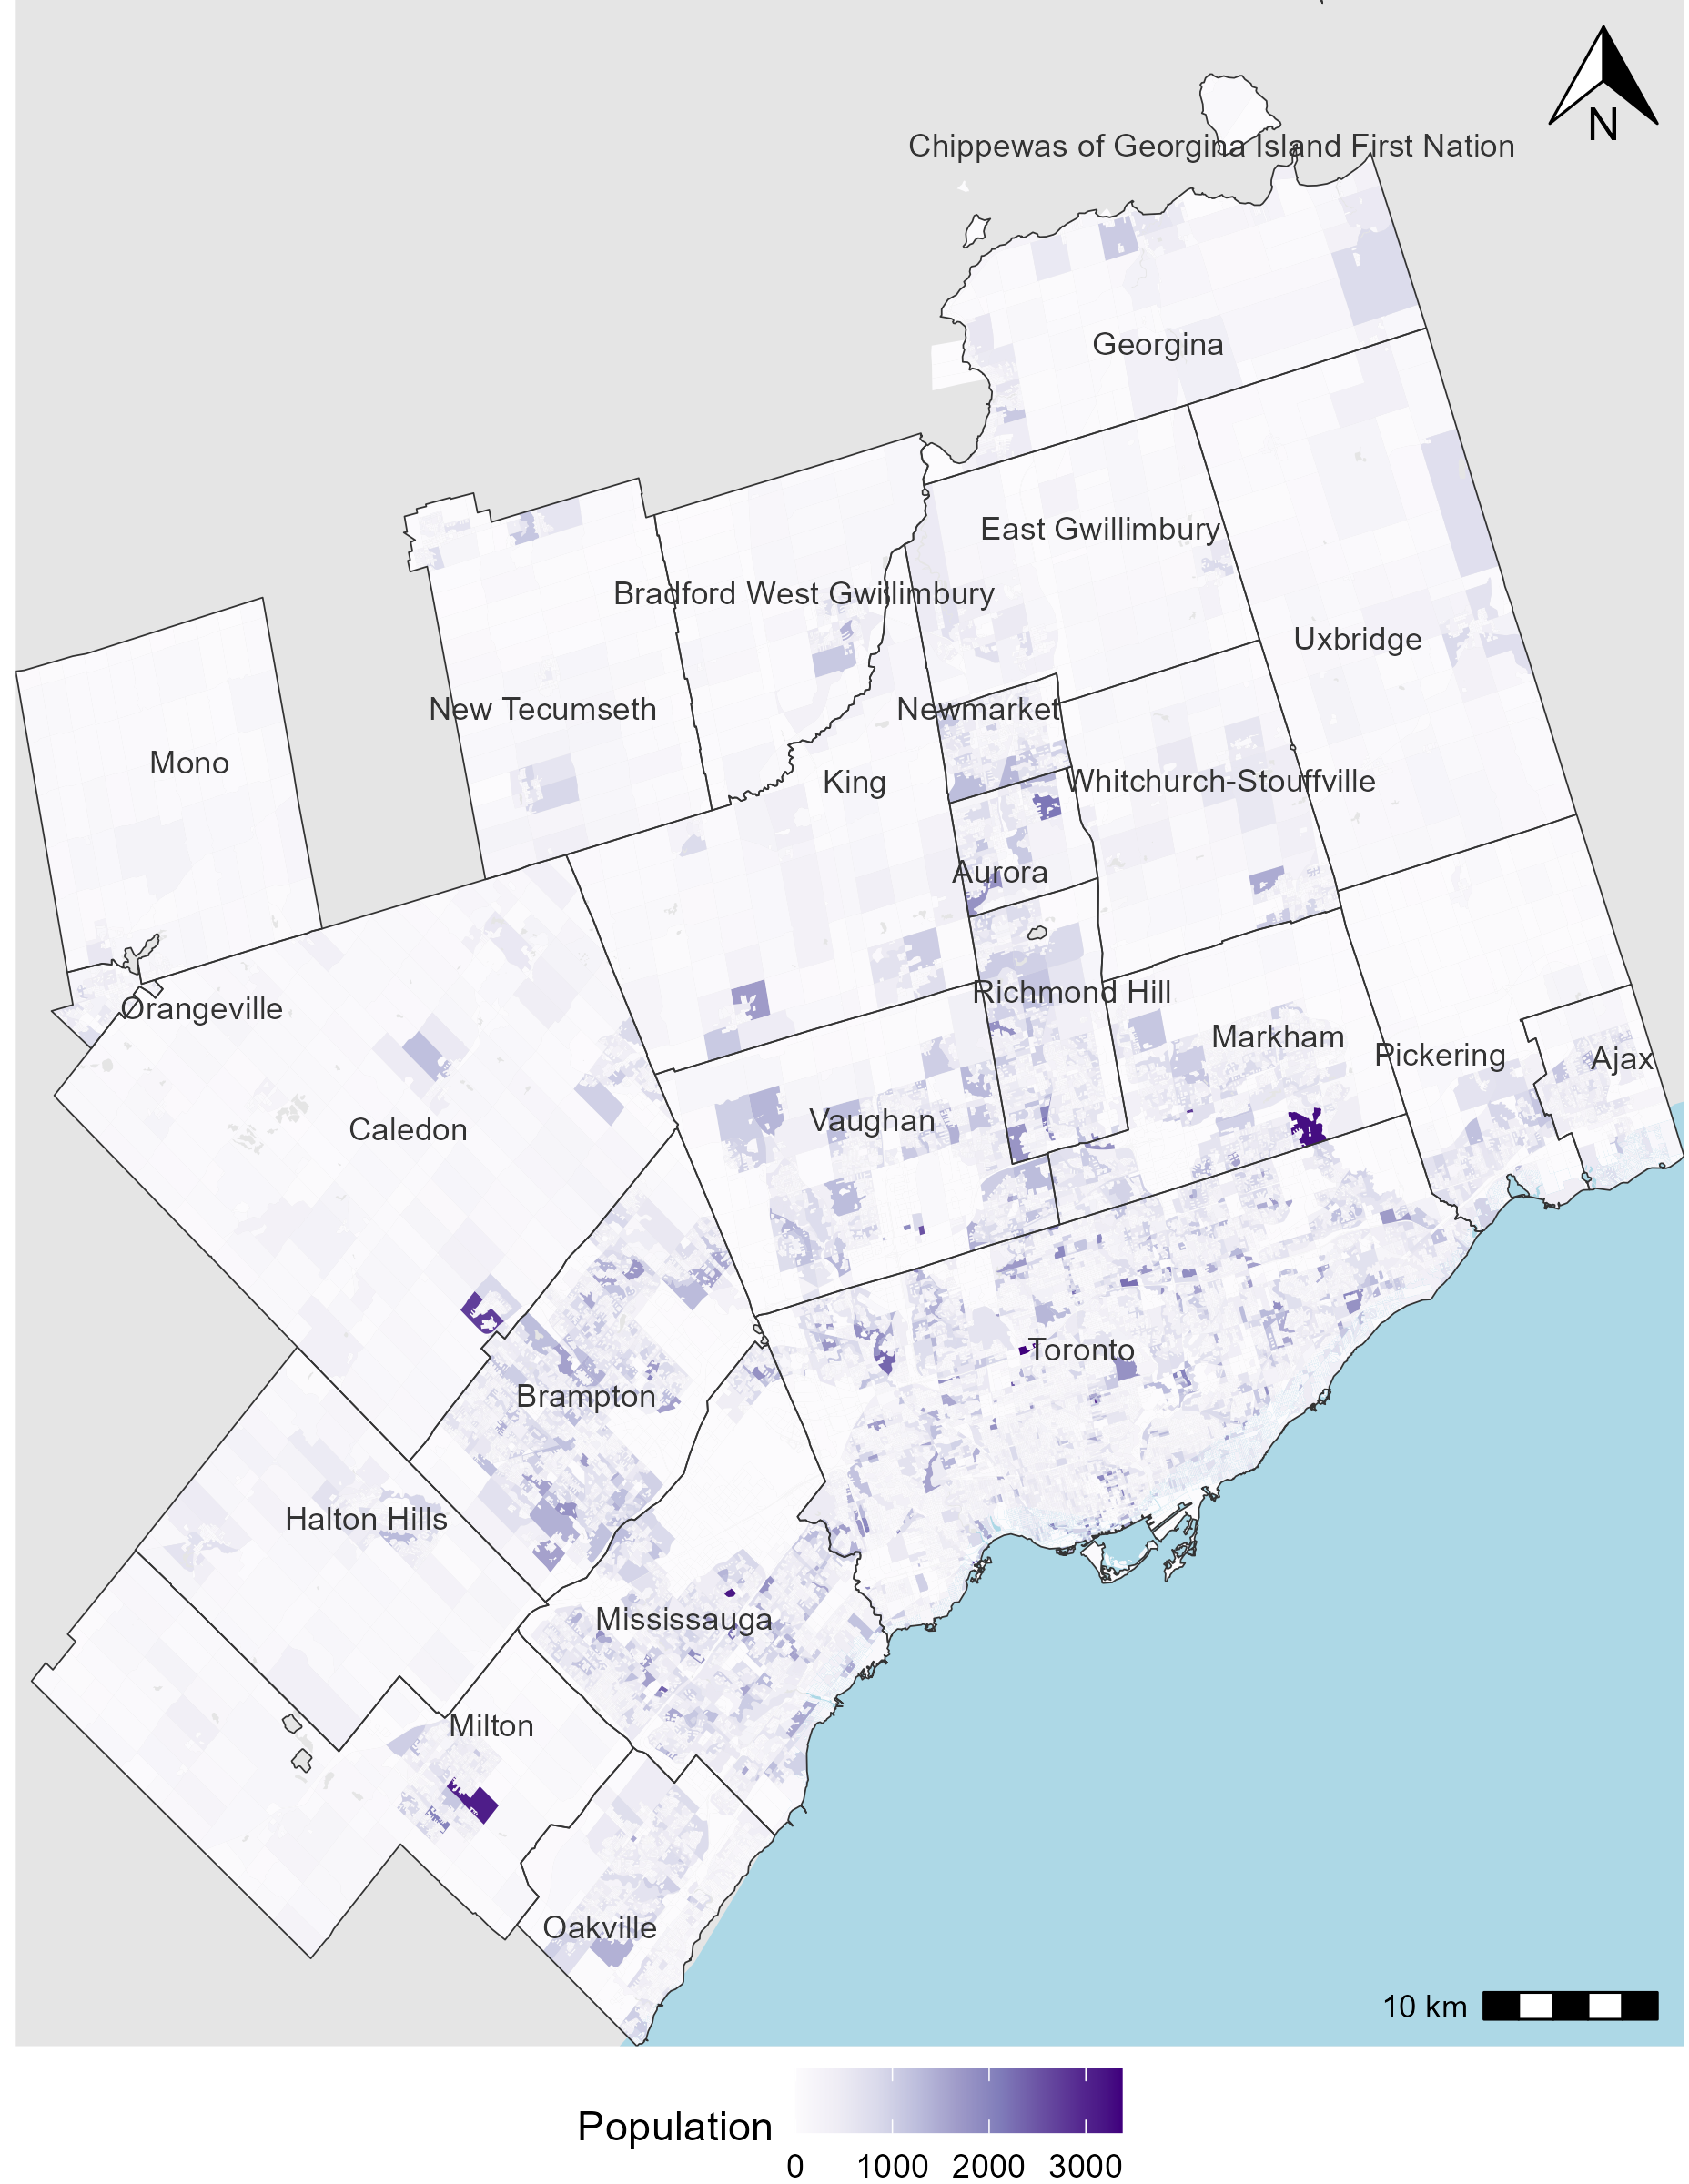
\includegraphics[width=6in]{./data/figures/chp2-toronto_CMA_plot} 

}

\caption{\label{fig:chp2-toronto_CMA_plot}Map of Toronto CMA with population per DB from the 2021 Census}\label{fig:unnamed-chunk-5}
\end{figure}

To contextualise the city of Toronto, the focus of this analysis, Figure \ref{fig:chp2-toronto_popden_NIAs_plot} demonstrates the 158 neighbourhoods in Toronto according to improvement classification: either a ``Neighbourhood Improvement Area'' (NIA), ``Emerging Neighbourhood'' (EA), or neither, based on an analysis conducted by the City. The methodology was based on the development of a composite indicator including dimensions of relative marginalization of the population who resides in these neighbourhood and of the neighbourhood infrastructure itself, such as variables reflecting economic opportunities (e.g., unemployment), social development (e.g., highschool graduation), participation in decision-making (e.g., voting), neighbourhood infrastructure (e.g., walkability, community places for meetings), and health (e.g., premature mortality) (City of Toronto, 2014, 2024). Overall, higher-population neighbourhoods are concentrated near the lake in the downtown core. Most NIAs are located in the east and northwest of the city and tend to have lower population densities, though two high-density NIAs are located in downtown.

\begin{figure}

{\centering 
\includegraphics[width=6in]{./data/figures/chp2-toronto_popden_NIAs_plot} 

}

\caption{\label{fig:chp2-toronto_popden_NIAs_plot}Map of the 158 Toronto neighbourhoods, with 'Improvement' classification and population density from the 2021 Census}\label{fig:unnamed-chunk-6}
\end{figure}

And lastly, the Figure \ref{fig:chp2-toronto_popden_DBCent_plot} displays the calculated DB weighted centroids, used as the origins in the accessibility analysis. There are 13322 points within the City, more spatially clustered in areas with higher population density.

\begin{figure}

{\centering 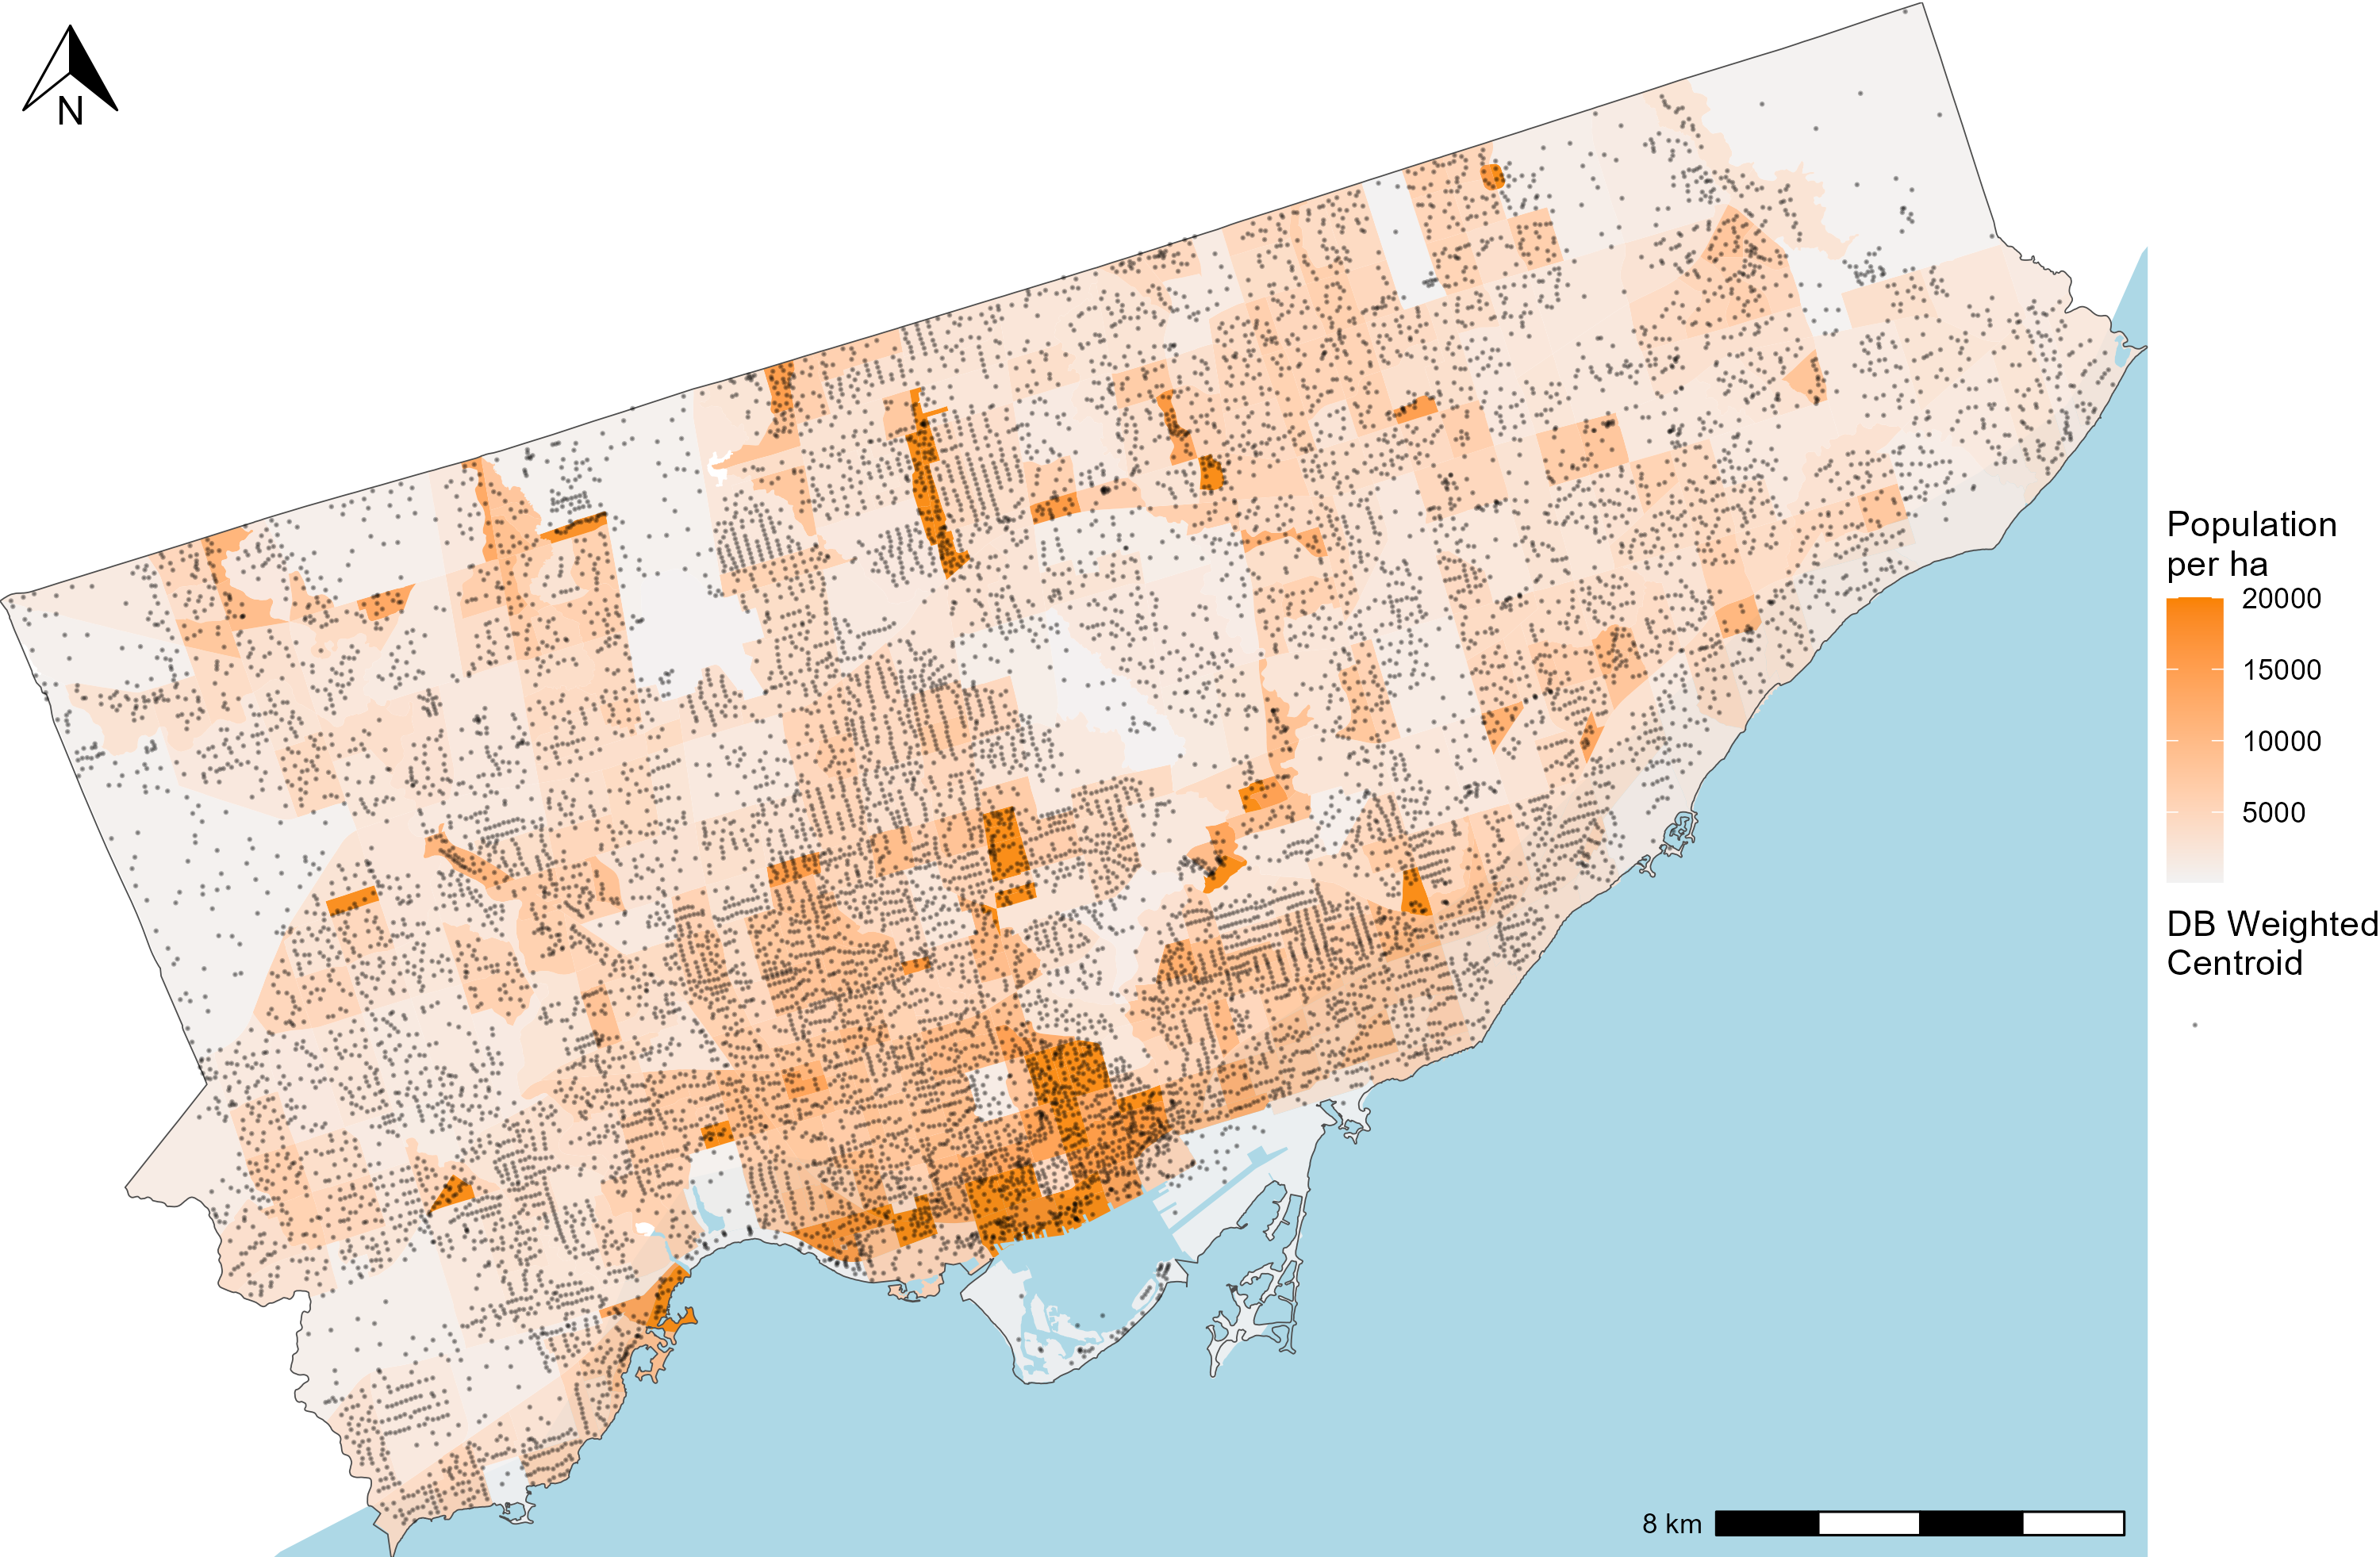
\includegraphics[width=6in]{./data/figures/chp2-toronto_popden_DBCent_plot} 

}

\caption{\label{fig:chp2-toronto_popden_DBCent_plot}Map of the City of Toronto's DB weighted centroids atop the population density from the 2021 Census}\label{fig:unnamed-chunk-7}
\end{figure}

\subsection{Toronto parkland destinations and normative travel behaviour}\label{toronto-parkland-destinations-and-normative-travel-behaviour}

Parkland is defined as city operated and/or owned `parks' identified in the greenspaces shapefile available through the city's official Open Data portal (City of Toronto, 2025). These are the same park assets that are identified as part of the Parkland Strategy report commissioned by the City of Toronto (City of Toronto, 2019, p. 20). This report serves as a guideline for assumptions made regarding park classification and interaction catchments based on park classification. Toronto's parkland is visualized in Figure \ref{fig:chp2-parkland_paths_plot}. Of note, other Open Spaces include in the greenspaces shapefile are federally or provincially owned/operated spaces, school yards, cemeteries, and hydro corridors. These spaces are not assumed to be Toronto operated and/or owned parkland, hence are not included in this analysis. These greenspaces are reflected as `no population' DBs.

\begin{figure}

{\centering 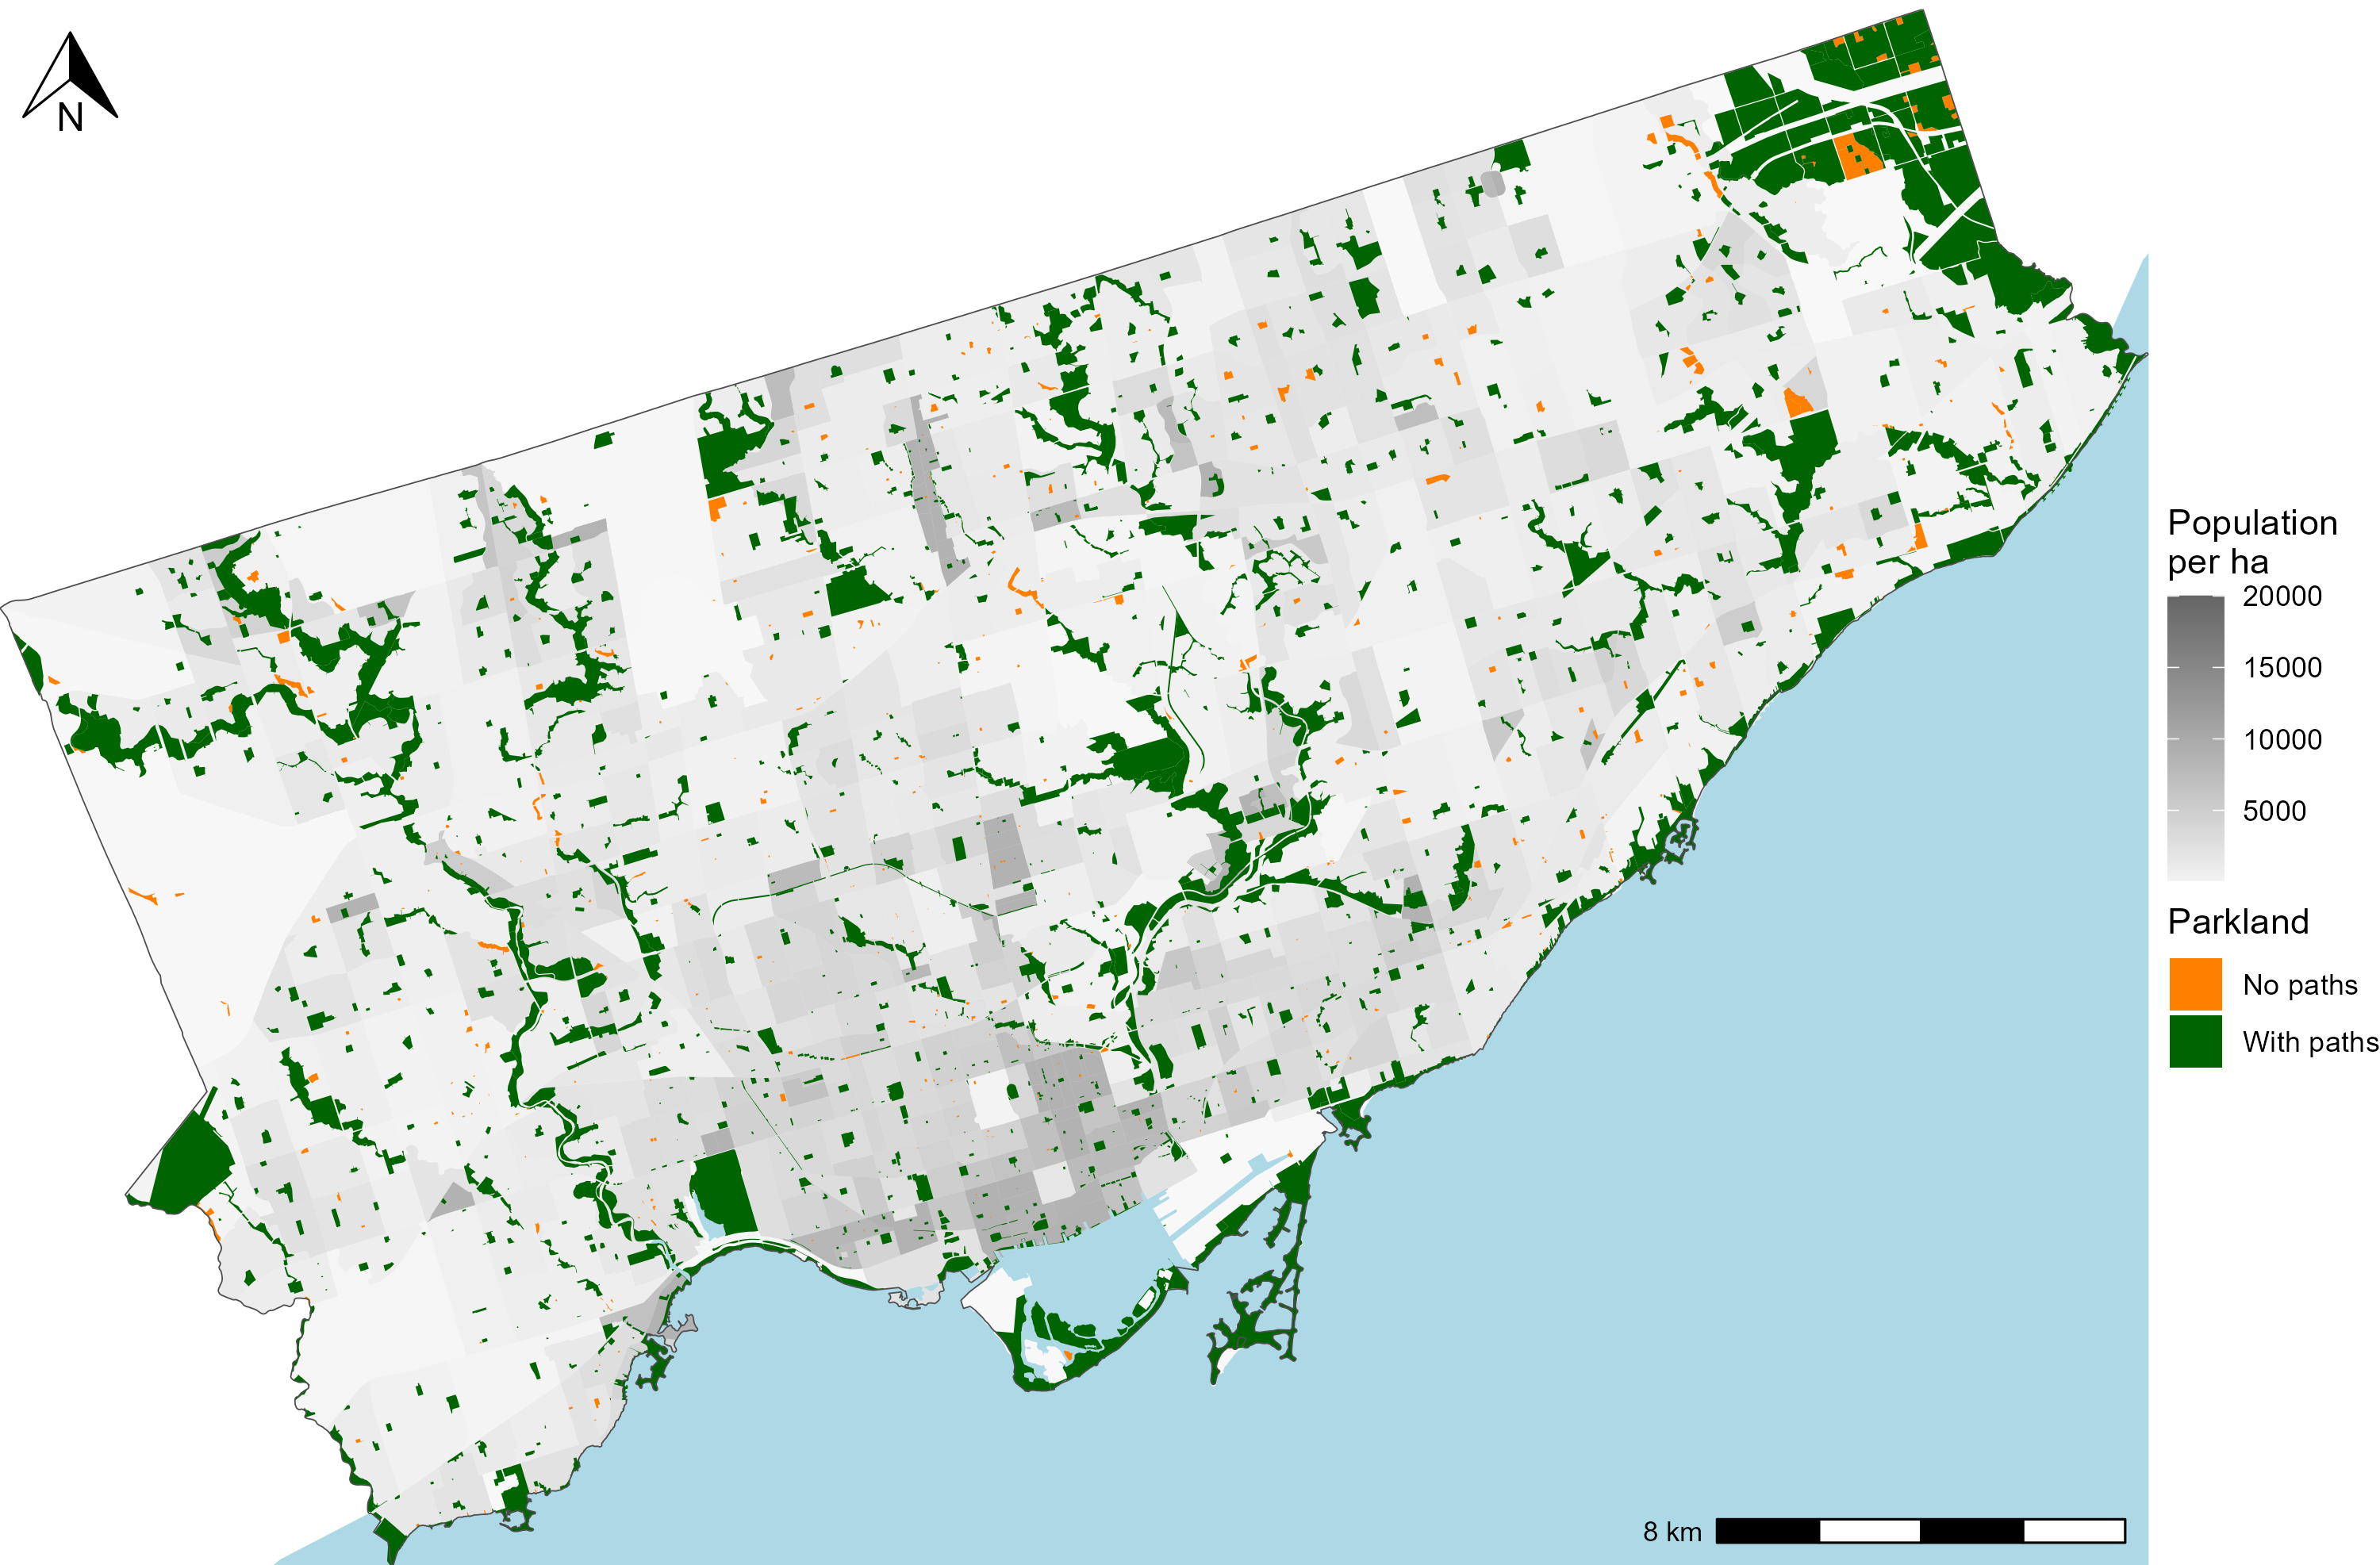
\includegraphics[width=6in]{./data/figures/chp2-parkland_paths_plot} 

}

\caption{\label{fig:chp2-parkland_paths_plot}Map of the City of Toronto's Parkland (with paths or no paths) atop the population density from the 2021 Census}\label{fig:unnamed-chunk-8}
\end{figure}

As retrieved from City of Toronto (2019, p. pg.15), the parkland can be categorized by size: `Parkette' (\textless0.5 ha) (40\% of all parks), `Small Park' (0.5--1.5 ha) (20\%), `Medium Park' (1.5--3.0 ha) 16\%, `Large Park' (3.0--5.0 ha) 9\%, `City Park' (5.0--8.0 ha) 5\%, and `Legacy Park' (\textgreater8.0 ha) 10\%. Interaction with parks can be assumed in a variety of ways, but in this analysis, it is normatively (Páez, Scott, \& Morency, 2012) assume interaction based on the park classification catchments described in City of Toronto (2019). Parkettes are assumed to only be accessible within a 10-minute travel window, small parks within 20 minutes, and medium parks within 30 minutes. In contrast, large, city, and legendary parks are considered to have citywide appeal, attracting people throughout the city regardless of travel time.

How parks can potentially be accessed is assumed based on their entrances. Entrances are not explicitly available, so they are assumed. They are calculated based on the parkland edge intersection with each path within the park itself or intersecting the park edge. 4 of the the 1607 parks have paths, each with anywhere between 1 to 84 (median of 2) entrances. The remaining 1603 parks do not have paths, and hence their entrances cannot be precisely assumed. Parks without an entrance are significantly smaller in area (i.e., median of 0.24 ha as opposed to the median of area parks with paths which is 1.43 ha). Upon visual inspection using Google Maps streetview, parks with no paths often contain a playground, some sport amenity or gardens within the center. Some of them are unfurnished -containing only mowed grass. For these parks with no internal paths, it is assumed then that these spaces can be entered from any direction and that the geometry centroid is the point of interest calculated and assumed as the entrance point. This point is snapped onto the transportation network based on an origin's shortest path, as will be later described in the routing subsection.

As a visualisation, Figure \ref{fig:chp2-park_entrance_example_plot} contains a panel of three DAs in Toronto, each displaying the roads, parks, and assumed park entrances. Readers should note that in the first two panels, these parks contain multiple entrance points, corresponding to where the edge of the paths within the parks intersect with the edge of the park boundary. These plots showcase different DAs that represent the diversity in DA size and park composition across the city. The first plot showcases a relatively small DA, near the downtown core of the city featuring high density of population, other amenities and multimodal transportation systems. This DA is unique in the area, as it features a large planned `Legacy' park by the name of Christie Pits. Planned parks are typically square or rectangular and can be accessed from most of the sides. They are also contained within the city in all areal sizes. The second plot contains a larger DA, north of downtown, that contains a few parks and near higher density suburban built form. One is the Roycroft Park Lands, a large `City' (smaller than Legacy), part of the Don River wetlands with maintained trails, enjoyed as nature reserve. Note it's long shape and minimal entrances. Natural parklands like Roycroft Park Lands are common along wetlands and other preserved natural spaces; they are typically larger in size (Medium, Large, or City parks) hence offer a lot of parkland space to those near their entrances. In the third plot, the DA is also large but with lower density suburban built form, and mostly residential. It contains only one small park: Pleasantview Park. This park contains no internal pathways, a playground in the middle of the park with no other amenities.

\begin{figure}

{\centering 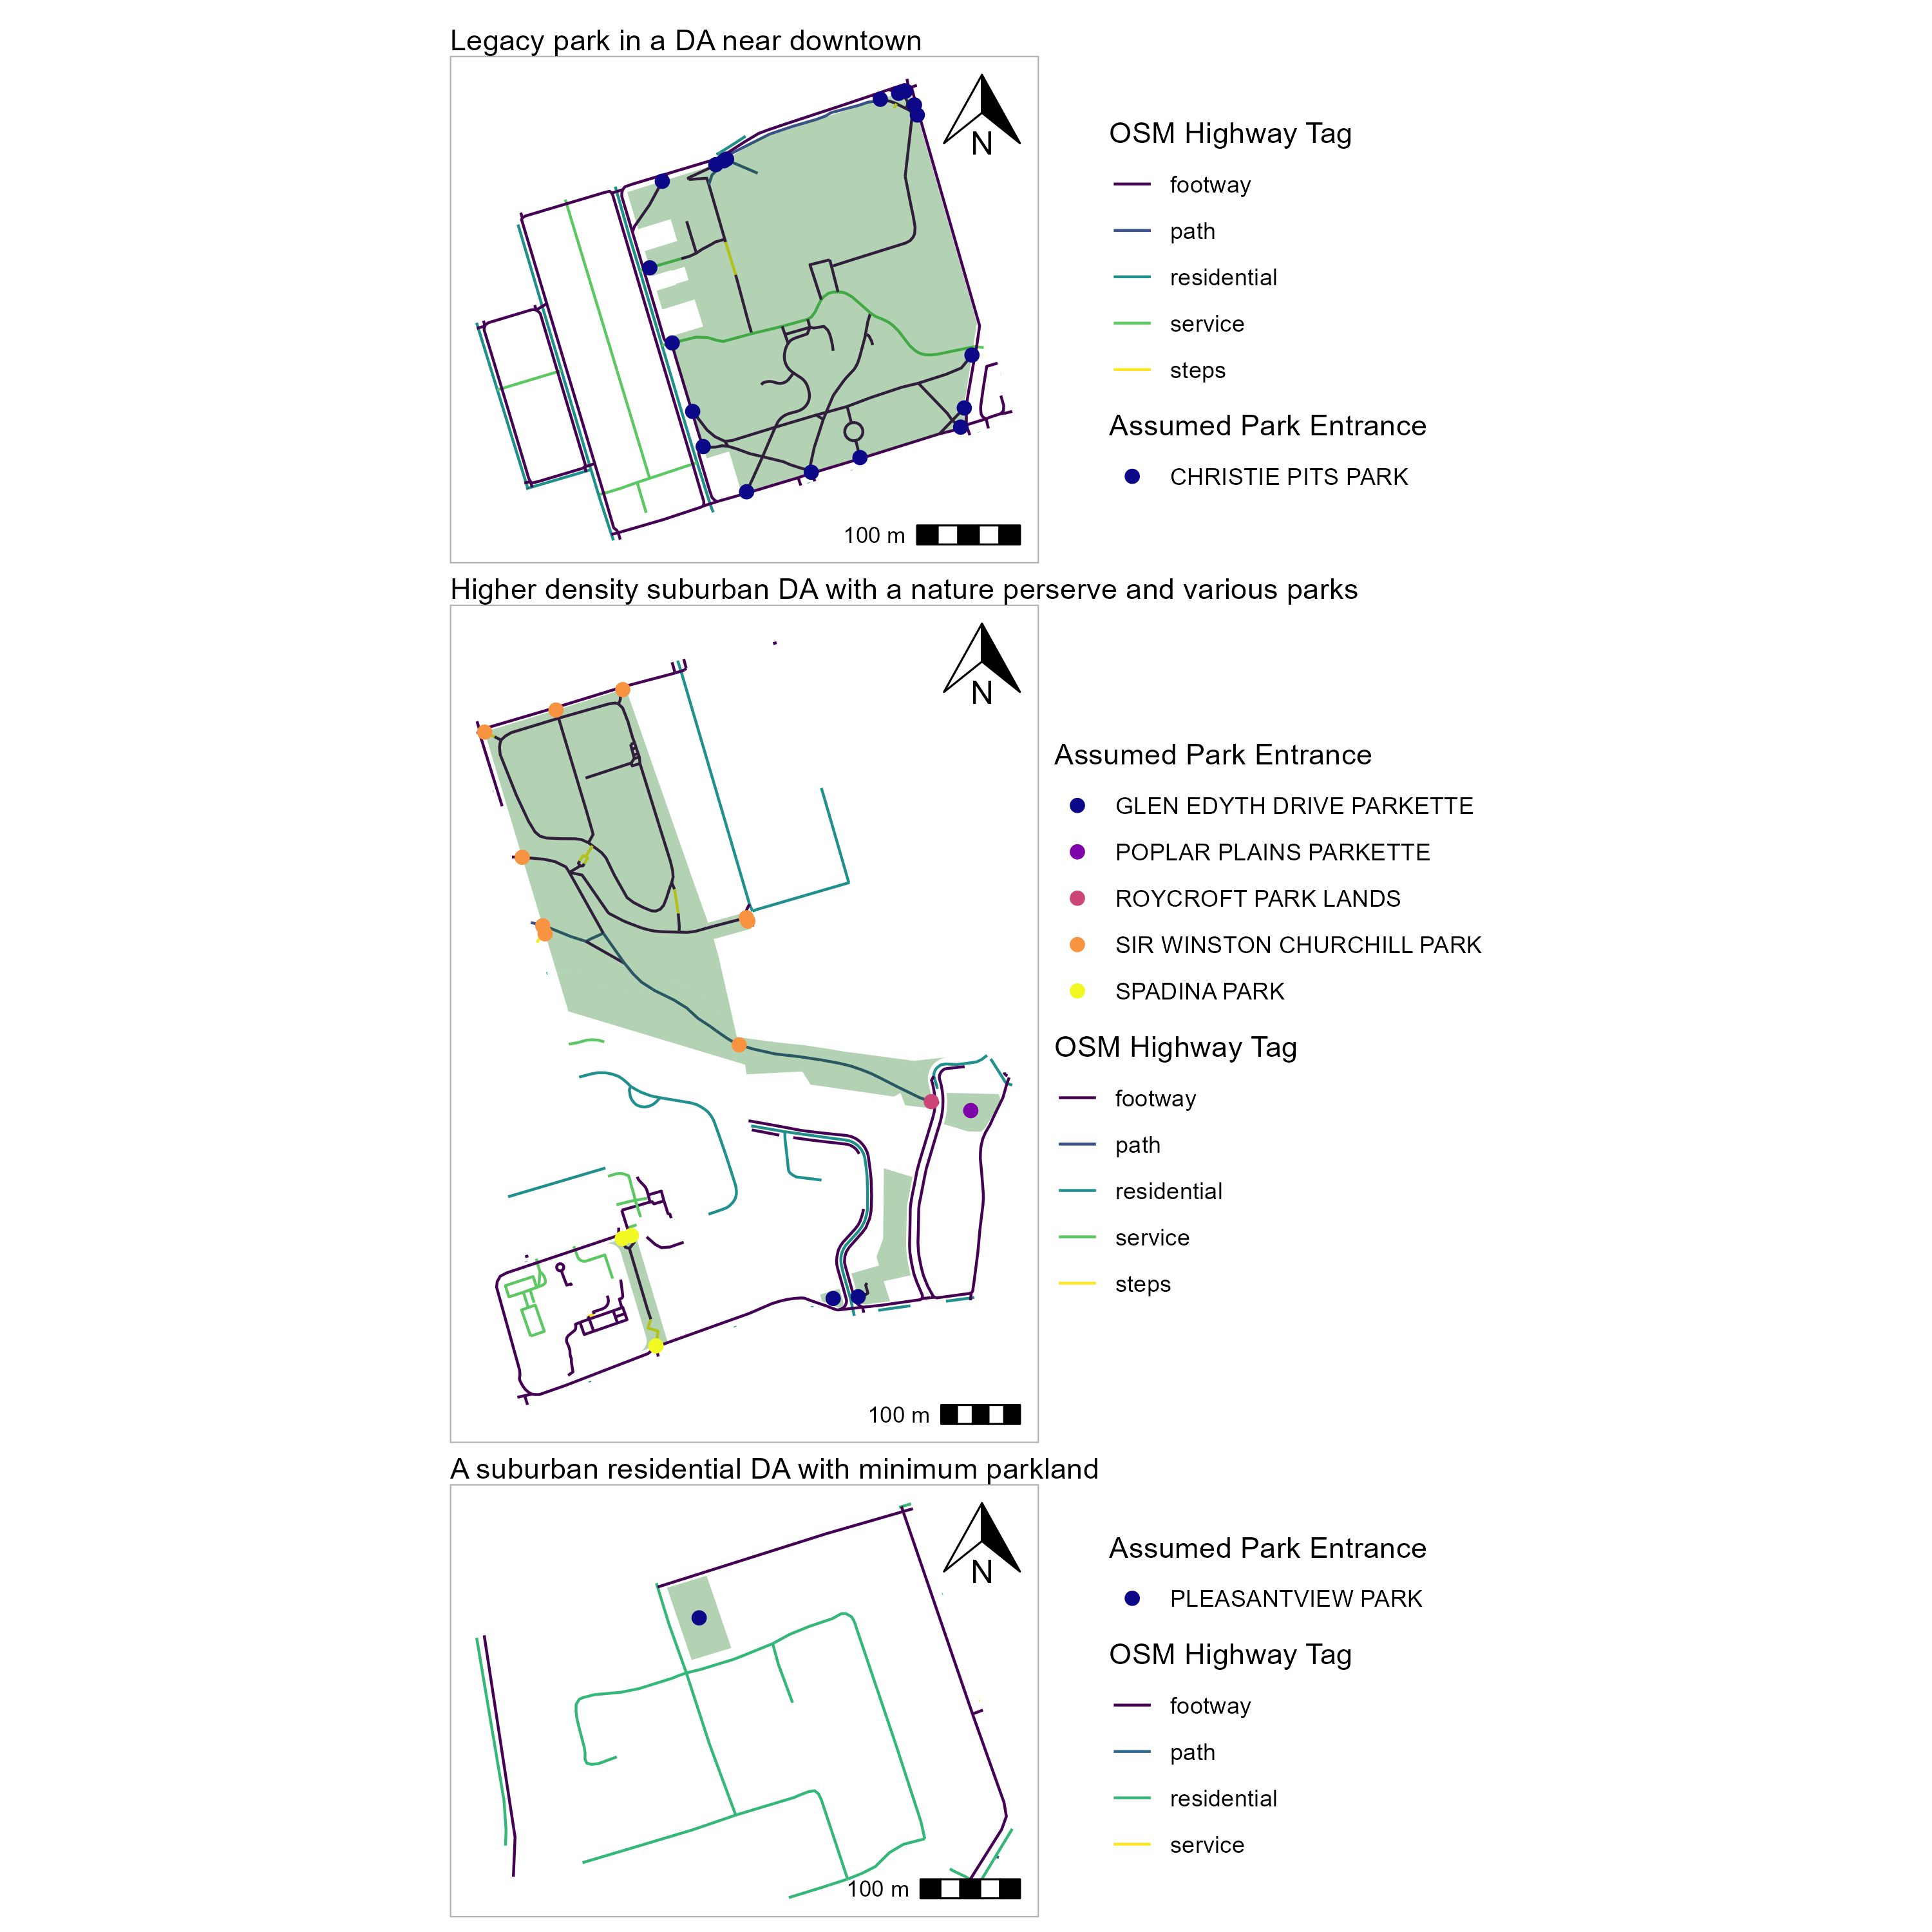
\includegraphics[width=6in]{./data/figures/chp2-park_entrance_example_plot} 

}

\caption{\label{fig:chp2-park_entrance_example_plot} Three DAs featuring parkland, road network by OSM tag, and park entrances. From top to bottom: planned Legacy park Christie Pits near the downtown core, parks north of the downtown core preserving natural space, and planned park with no paths in a more suburban DA.}\label{fig:unnamed-chunk-9}
\end{figure}

\subsection{Multimodal origin to destination routing and trip lengths}\label{multimodal-origin-to-destination-routing-and-trip-lengths}

Routing of travel times was done using the travel\_time\_matrix() function in \{r5r\}, an R package that provides an R-interface for the Java-based R5 Routing engine (Pereira, Saraiva, Herszenhut, Braga, \& Conway, 2021). The function was run four time, one for bicycle, car, transit and walking modes, producing four separate travel time matrices. Each origin destination pair has an associated shortest travel time, selected by the function based on all possible origin destination routes given the input road network (and transit schedule, for the transit mode). The road network is an edited version of OpenStreetMaps (OSM) street network (December 9, 2022) and edited General Transit Feed Specification (GTFS) files (February 4, 2024) for transit operating within the City i.e., GO (regional commuter train and bus service), TTC (local subway, lightrail, and bus network), and the UP Express (regional commuter train line). The files were edited by city staff to more accurately reflect access into TTC subway stations and reflect the transit schedule for the week of February 4 2025.

Concerning the inputs for the `travel\_time\_matrix()' function for all modal travel time calculations: the origins are the DB weighted centroids (13322 locations), the destinations are points representing the 1607 parks and the OSM road network were used. Some parks have multiple pieces, separated by the road network: in total, there are 1958 park pieces, each with between 1 and 68 path entrances (median 3 entrances) or 1 park piece centroid. In total, there are 6274 possible destination points (5724 path entrances and 550 centroids) for each of the 13322 origins.

For the motorized modes, a maximum travel time of 120 minutes was selected. For transit, the GTFS files and a departure time of between 11:00-11:15am (i.e., a 15 minute departure window) on February 8th 2025 was used, to reflect a Saturday afternoon transit schedule. Travel speeds reflect the posted speeds and intersections as gleaned from the OSM road network, and for transit, the scheduled transit arrival times at stops according to the GTFS file. For non-motorized modes, a maximum travel time of 30 minutes was selected, and the default travel speeds of 3.6 km/h for walk and 12 km/h for cycling was assumed. The travel time thresholds of 120 minutes and 30 minutes was set to normatively reflect the likelihood to travel to parks, by mode.

It is worthwhile summarising the multimodal travel time matrices. Notably, within a 120 minutes trip by motorized modes, the majority of DBs can reach all parks by car (with exception to the 6 on the Toronto Islands, inaccessible by car), i.e., the median DB can reach 1601 out of the 1607 parks, while the most isolated can still reach 184 parks. By contrast, within a 120 minute trip or less by transit, a median DB can only reach 1116 parks, with the most central DB reaching 1539 parks meaning 4\% of parks are feasibly unreachable by transit for DBs in the City of Toronto. These parks are located at the edges of the city in that are transit poor, as will be demonstrated and discussed in the findings. Comparing this reach to the lower range non-motorized modes, the number of parks reachable by foot or by cycle within 30 minutes from a DB is much lower: a median DB can only reach 15 parks (max. 61 parks for the most central DB) by walking and 86 parks (max. 295 parks for the most central DB) by cycling.

As a final note on routing assumptions, it's useful to compare travel times to park centroids versus park path entrances. For the 1204 parks with known path entrances, centroids were also computed and travel times from all DBs to all centroids were calculated. This comparison highlights the impact of the R5 routing algorithm, namely, how the routed travel times can differ depending on how the destination points are `snapped' to the nearest road segment. If a point is not already on the road network, R5 snaps it to the nearest network segment, adding a walking time penalty based on distance. This snapping algorithm prioritizes minimizing overall travel time from the origin. Since edge entrances are typically already on the network, their snapping penalty is minimal. In contrast, centroid points--especially in large and irregular natural parks---may snap to parts of the road network that are unreachable by certain roads (e.g., far enough away from bus stops, or bike lanes), inflating travel times. Hence: when paths within the parks are available from the OSM network, they are used, as it more accurately reflects the points at each the parks can actually be entered from. But when the park has no entrances, it is assumed that the centroid (or the middle of the park itself) is the destination point, and the associated snapping penalty is folded into the calculated travel time. The following Figure \ref{fig:chp2-ent_vs_cent_tt_car_transit_scatter} and Figure \ref{fig:chp2-ent_vs_cent_tt_cycle_walk_scatter} demonstrate the relationship between the minimum travel time used in the analysis for each parks with path entrances and the travel time if its centroid point was used, along with a 45 degree dashed line representing a perfect linear relationship.

Regarding the motorized modes in Figure \ref{fig:chp2-ent_vs_cent_tt_car_transit_scatter}), the relationship appears to be roughly, with centroid times being consistently lower than path entrance times--except for a few parks that fall to the left of the dashed line. Parks with entrance times that are larger than their centroid times have entrances that are not in opportune positions on the network relative to the snapped centroid point, and vice versa for entrances that have \emph{lower} travel times than their centroid points which is often the case. Transit shows a similar trend but with more noise. A few parks exhibit exceptionally high transit times relative to their centroid times. These are typically larger parks where the centroid snaps to a location near access points to the transit system, but the \emph{actual} path entrances are not in proximity to those opportune system access point. Since the road network for cars is more continuous and the system is more evenly accessible (e.g., the majority of roads can be driven on, whereas the transit system can only be entered in specific points), this discrepancy is not observed in the car mode. This comparison underscores the importance of using realistic entrance points especially for larger parks with few entrance points and for modes like transit, which do not provide uniform access into the system.

\begin{figure}

{\centering 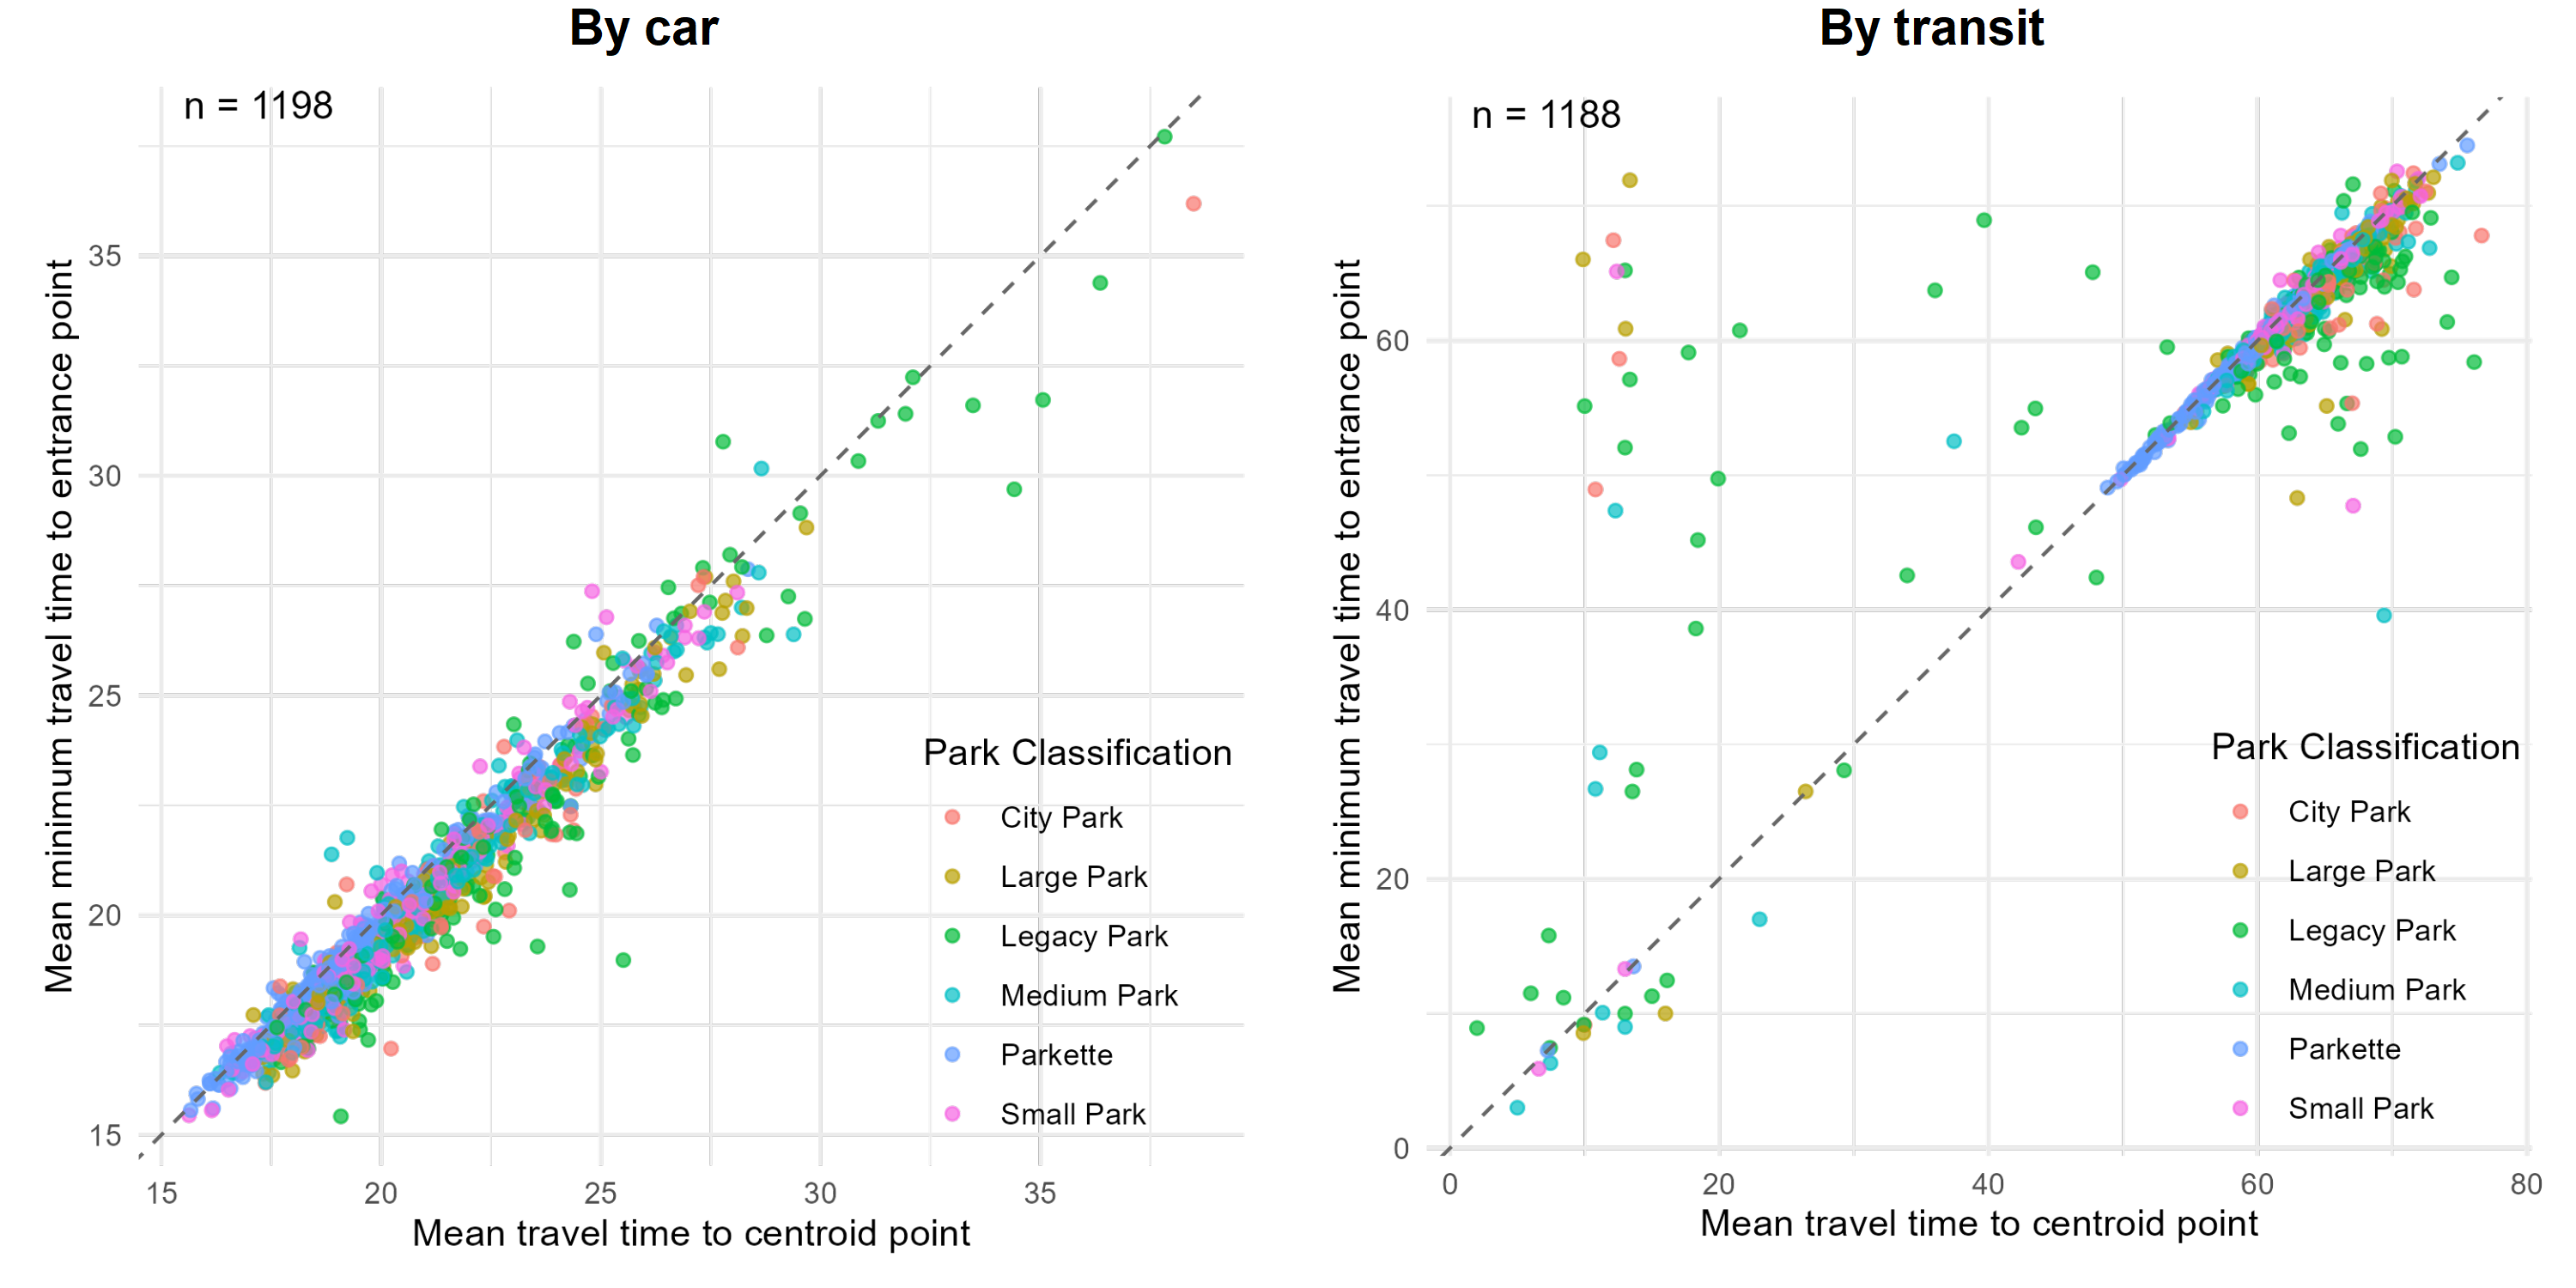
\includegraphics[width=6in]{./data/figures/chp2-ent_vs_cent_tt_transit_car_scatter} 

}

\caption{\label{fig:chp2-ent_vs_cent_tt_car_transit_scatter} Scatter plot of car and transit travel times from origins to destinations by destination type for each park (either mininum median travel time to park centroid, or minimum median travel time to park entrance). }\label{fig:unnamed-chunk-10}
\end{figure}

Figure \ref{fig:chp2-ent_vs_cent_tt_cycle_walk_scatter} captures the non-motorized modes, which exemplifies a similar pattern as the motorized modes, with centroid travel times beign typically longer than path entrance points in a linear relationship. However, like transit and car, travel by bike and walk demonstrate different levels of noise. As the travel time threshold is 30 minutes, distance can be traversed at a faster rate by bike than by foot, hence differences in distances between the path entrance point and the snapped centroid is less impact on the estimated travel time for bike mode.

\begin{figure}

{\centering 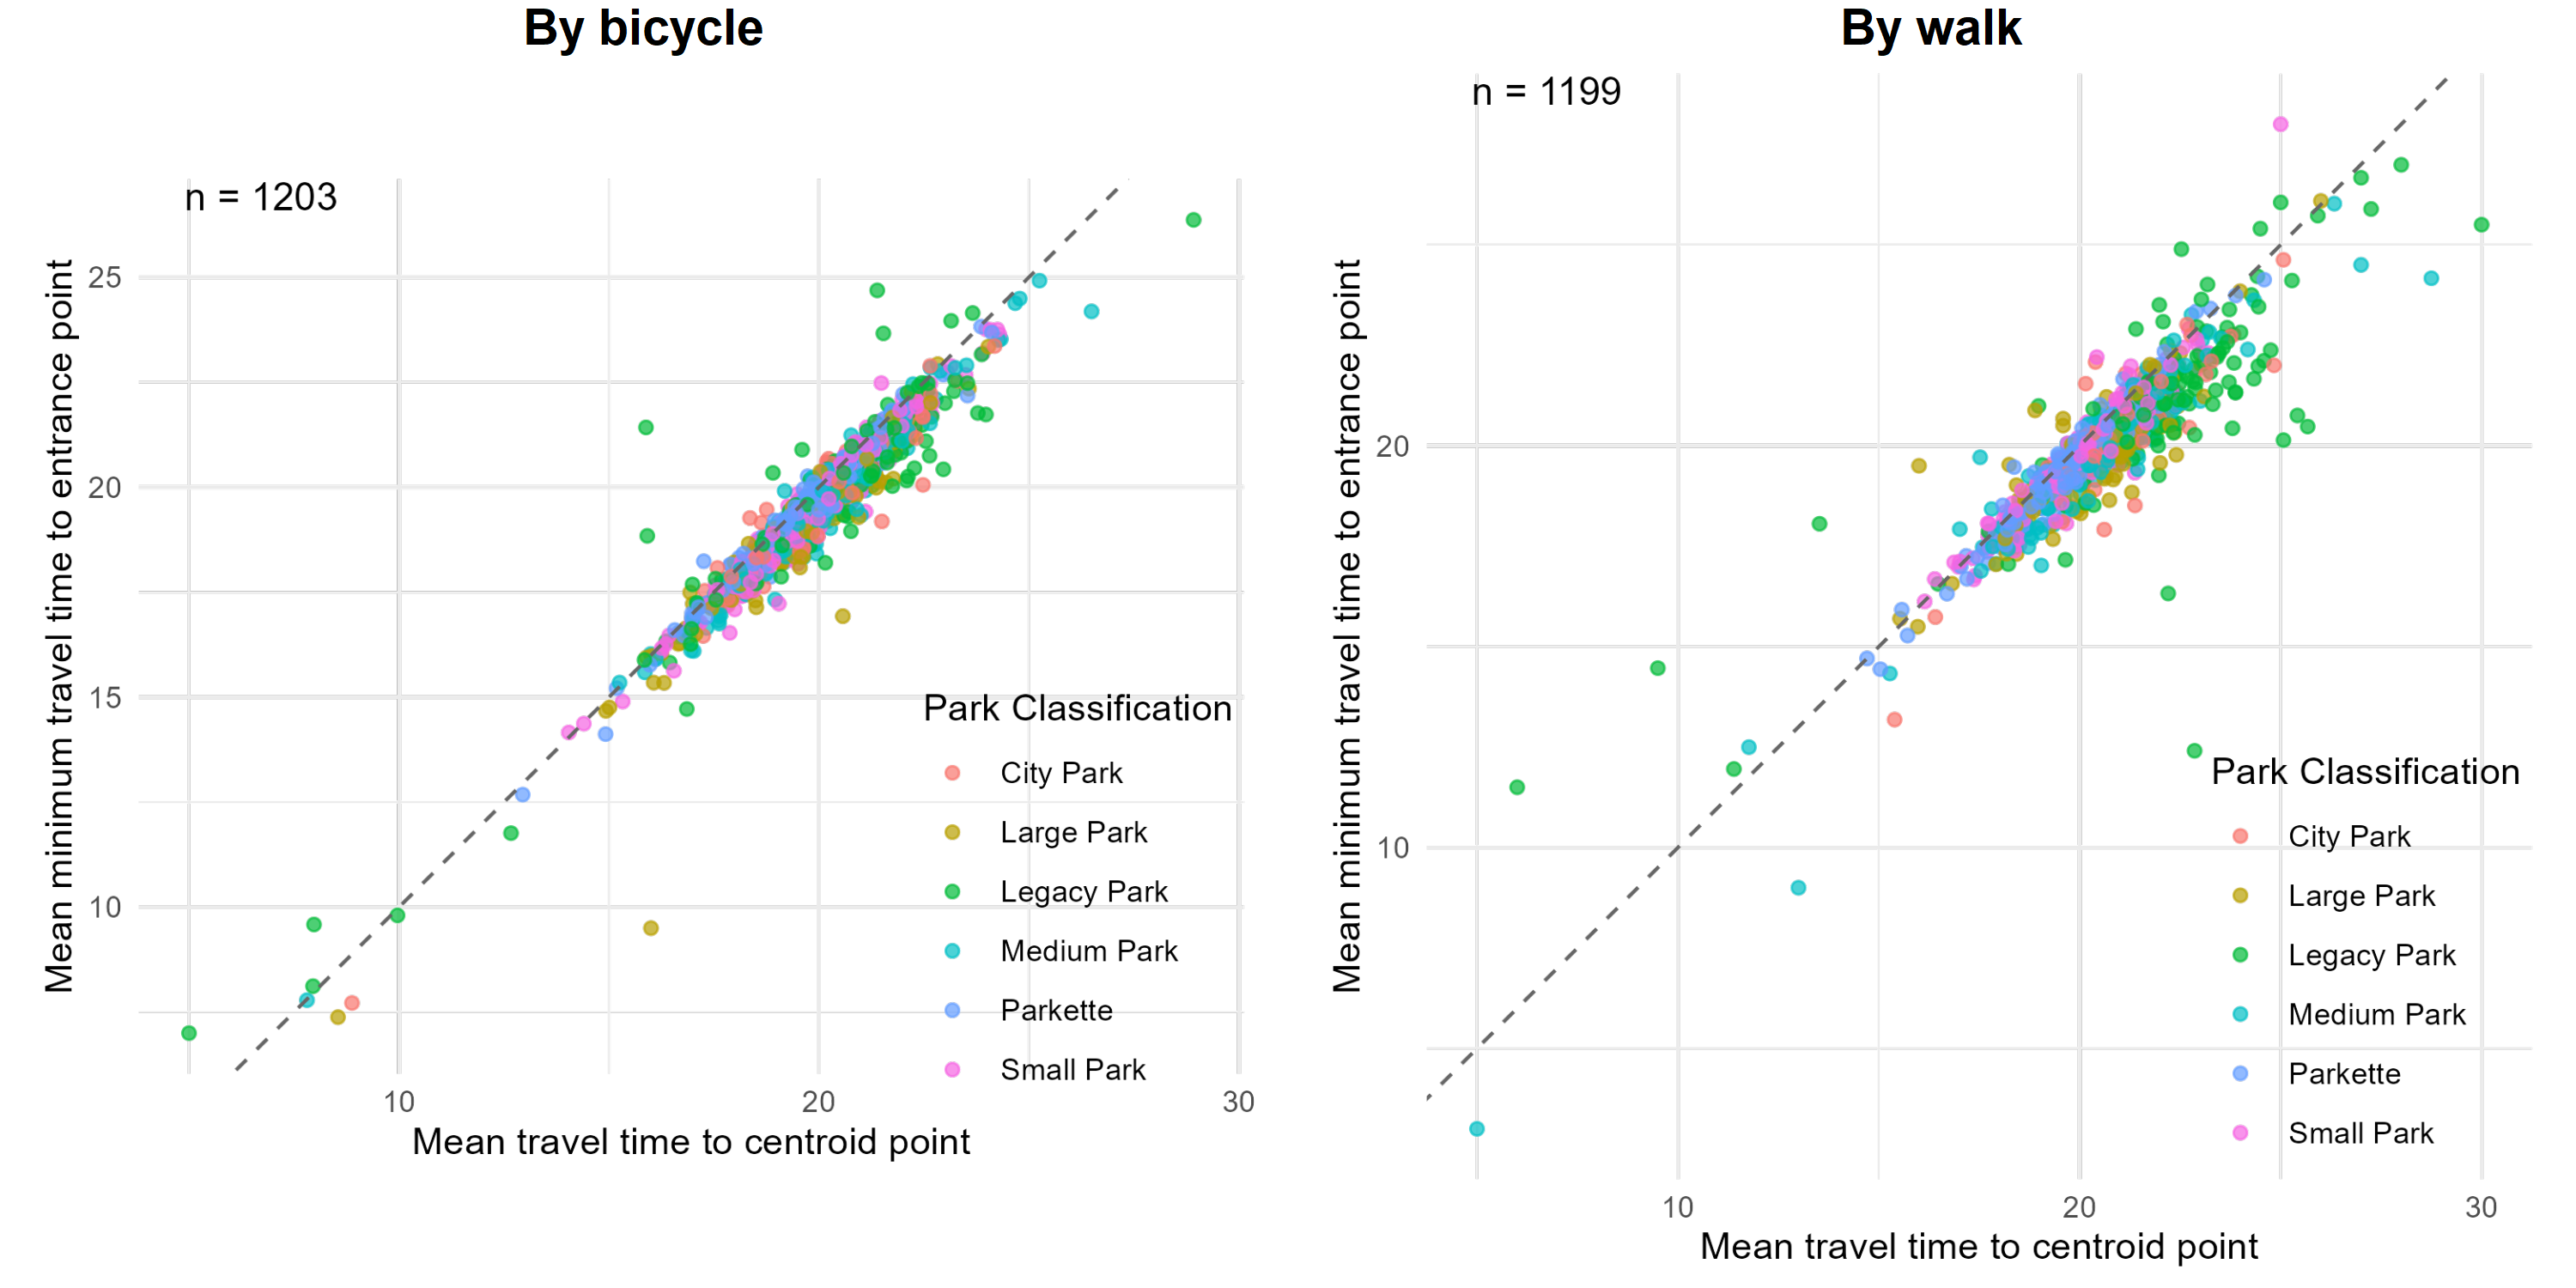
\includegraphics[width=6in]{./data/figures/chp2-ent_vs_cent_tt_walk_cycle_scatter} 

}

\caption{\label{fig:chp2-ent_vs_cent_tt_cycle_walk_scatter}  Scatter plot of cycle and walk travel times from origins to destinations by destination type for each park (either min mean travel time to park centroid, or to min mean travel time to park entrance). }\label{fig:unnamed-chunk-11}
\end{figure}

\subsubsection{Normative park trip length}\label{normative-park-trip-length}

A key component of accessibility is how the cost of overcoming spatial separation to reach a destination is considered. In this analysis, access to parkland is modeled using distance catchments based on park size classifications from the City of Toronto (2019) report, and modal options informed by discussions with city staff.

It is assumed that the smaller parks, i.e., parkette (\textless0.5ha), small parks (0.5-1.0 ha), and medium parks (1.5-3 ha) offer a service coverage of only 0.5km, 1.0km and 1.5km, respectively. Meaning, people are only likely to interact with the park within this travel distance. This assumption has to do with the qualities these parks possess, and the availability of similar parks in the area: namely, these smaller parks are often located in residential neighbourhoods, evenly spatially distributed, and often offer no exceptional amenity that can't be substituted by another similarly sized park nearby as inferred from City of Toronto (2019). For larger parks, such as large parks (3-5 ha), city parks, and legacy parks, their service catchments are larger as they are more unique, attractive, and harder to substitute parks, as inferred from the City of Toronto (2019) report. Large parks are assumed a service coverage of 3km and city and legacy parks are assumed to be attractive, and hence cover, the whole city.

\begin{verbatim}
[1] 17.12376
\end{verbatim}

Trip lengths to parks vary by both travel mode and park classification. Based on assumptions drawn from City of Toronto (2019) and discussions with city staff, travel impedance functions are created based on trip lengths that are \emph{seen} as acceptable. It is assumed that (1) non-motorized travelers can access all parks based on their service coverage catchment (i.e., a 0.5 km catchment for parkettes that translate to 8 mins of walking or 3 mins of cycling based on median travel speeds), however, they are constrained by their maximum travel time length of 30 minutes. (2) transit users can access all types of parks, but based on a negative exponential distance decay function (\(f(c_{ij}) = e^{-0.02c_{ij}}\)). This function has a median travel time of approximately 30 minutes, meaning that half of the total weight of the travel impedance function--representing the spatial separation between people and parks--comes from trips between 0 to 30 minutes, and the other half comes from trips between 30 to 120 minutes. The function captures the idea that the deterrent effect of distance increases gradually, assigning progressively less `spatial interaction' weight to more distant parks, even though they remain reachable. (3) Car users are assumed \emph{not} to travel to smaller parks at all, and as such, these parks are excluded from accessibiltiy results for the car mode. For larger parks, car travel impedance is assumed also based on a negative exponential distance decay function, but with parameter \(-0.04\) (\(f(c_{ij}) = e^{-0.04c_{ij}}\)), twice as steep as the transit impedance function. This reflects a stronger deterrent effect with increasing travel time. Namely, with a median travel time of approximately 17 minutes, trips that are between 0 to 17 minutes are assigned half the weight of the travel impedance function and the remaining half is defused acrossed trips that are between 17 minutes to 60 minutes. Destinations 60 minutes are considered effectively unreachable, with the function modeled as 0 beyond this point.

These assumptions on interaction with parks and trip lengths by mode have equity implications:
- Smaller parks are assumed to only be attractive to, hence accessible for, non-motorized and transit users
- For larger parks which can be reached by all modes, car mode has the largest range and has a steep decay, meaning it may provide favourable spatial seperation weight, relative to other modes.
- Travel impedance for transit users is penalized more gradually, assuming broader reach to all park types
- Non-motorized users reach is constrained practically: they are assumed not to travel beyond 30 minutes
- For parks in less densely populated areas, i.e., with travel times by sustainable modes beyond 30 minutes, accessibility will only be present for car users. In sum, individuals in these areas who do not have access to a vehicle are effectively excluded.

These assumptions on interaction with parks and trip lengths by mode have equity implications:
- Smaller parks are assumed to be attractive only to non-motorized and transit users, and are therefore not included in the accessibility profile for car users.
- For larger parks, which are accessible by all modes, the car mode has the broadest assumed range and steepest decay, potentially resulting in more opportune spatial separation weighting relative to other modes.
- Transit users face a more gradual decay in travel impedance, reflecting broader assumed reach across all park types.
- Non-motorized users are assumed to be practically constrained in their reach, with travel limited to within 30 minutes on foot or by bike.
- Parks in lower-density areas requiring more than 30 minutes of travel by sustainable modes will contribute to high accessibility for car users exclusively. Individuals in these areas without access to a private vehicle are, effectively, excluded, and these zones will reflect very low levels of accessibility by sustainable modes.

To summarise the modal \(m\) travel behaviour based on parkland classification type \(y\) as the resulting travel impedance functions \(f^m(c^m_{ij})\) in Table \ref{tab:chp2-travel-impedance-by-park-mode}:

\begin{table}[ht]
\centering
\small
\begin{tabular}{|l|c|c|c|c|}
\hline
\textbf{Park Type} & \textbf{Car} & \textbf{Transit} & \textbf{Cycling} & \textbf{Walking} \\
\hline
Parkette &
0 &
$e^{-0.02} \cdot c_{ij}^{\text{transit}}$ &
$1$ if $c \leq 3$ min, else 0 &
$1$ if $c \leq 8$ min, else 0 \\
\hline
Small Park &
0 &
$e^{-0.02} \cdot c_{ij}^{\text{transit}}$ &
$1$ if $c \leq 5$ min, else 0 &
$1$ if $c \leq 17$ min, else 0 \\
\hline
Medium Park &
0 &
$e^{-0.02} \cdot c_{ij}^{\text{transit}}$ &
$1$ if $c \leq 8$ min, else 0 &
$1$ if $c \leq 25$ min, else 0 \\
\hline
Large Park &
$e^{-0.04} \cdot c_{ij}^{\text{car}}$ &
$e^{-0.02} \cdot c_{ij}^{\text{transit}}$ &
$1$ if $c \leq 15$ min, else 0 &
$1$ if $c \leq 30$ min, else 0 \\
\hline
City Park &
$e^{-0.04} \cdot c_{ij}^{\text{car}}$ &
$e^{-0.02} \cdot c_{ij}^{\text{transit}}$ &
$1$ if $c \leq 30$ min, else 0 &
$1$ if $c \leq 30$ min, else 0 \\
\hline
Legacy Park &
$e^{-0.04} \cdot c_{ij}^{\text{car}}$ &
$e^{-0.02} \cdot c_{ij}^{\text{transit}}$ &
$1$ if $c \leq 30$ min, else 0 &
$1$ if $c \leq 30$ min, else 0 \\
\hline
\end{tabular}
\caption{Normative travel impedance functions by parkland classification $y$ and mode $m$}
\label{tab:chp2-travel-impedance-by-park-mode}
\end{table}

To reiterate, the trip length based travel time behaviour summarised in Table \ref{tab:chp2-travel-impedance-by-park-mode} are \emph{normative}--they represent a statement about what should be considered a reasonable travel time that defines parkland accessibility (Páez et al., 2012). In practice, however, travel behaviour empirically may diverge from these normative statements. For example, empirical data from the 2023 Transportation Tomorrow Survey of trips made for `leisure' purposes by different modes in the Greater Toronto Area region, reveals different patterns (Data Management Group, 2023). Figure \ref{fig:chp2-norm_pos_impedance_mode_parktype_plot} compares this normative travel behaviour (green lines) from Table \ref{tab:chp2-travel-impedance-by-park-mode} with the TTS empirically derived curves (dashed lines). For this analysis, the normative curves (i.e., Table \ref{tab:chp2-travel-impedance-by-park-mode}) are used to define accessibility. This will enable the interpretation of results in terms of what \emph{should} be accessible via each mode, according to planning goals, rather than what currently is based on observed travel behaviour.

\begin{figure}

{\centering 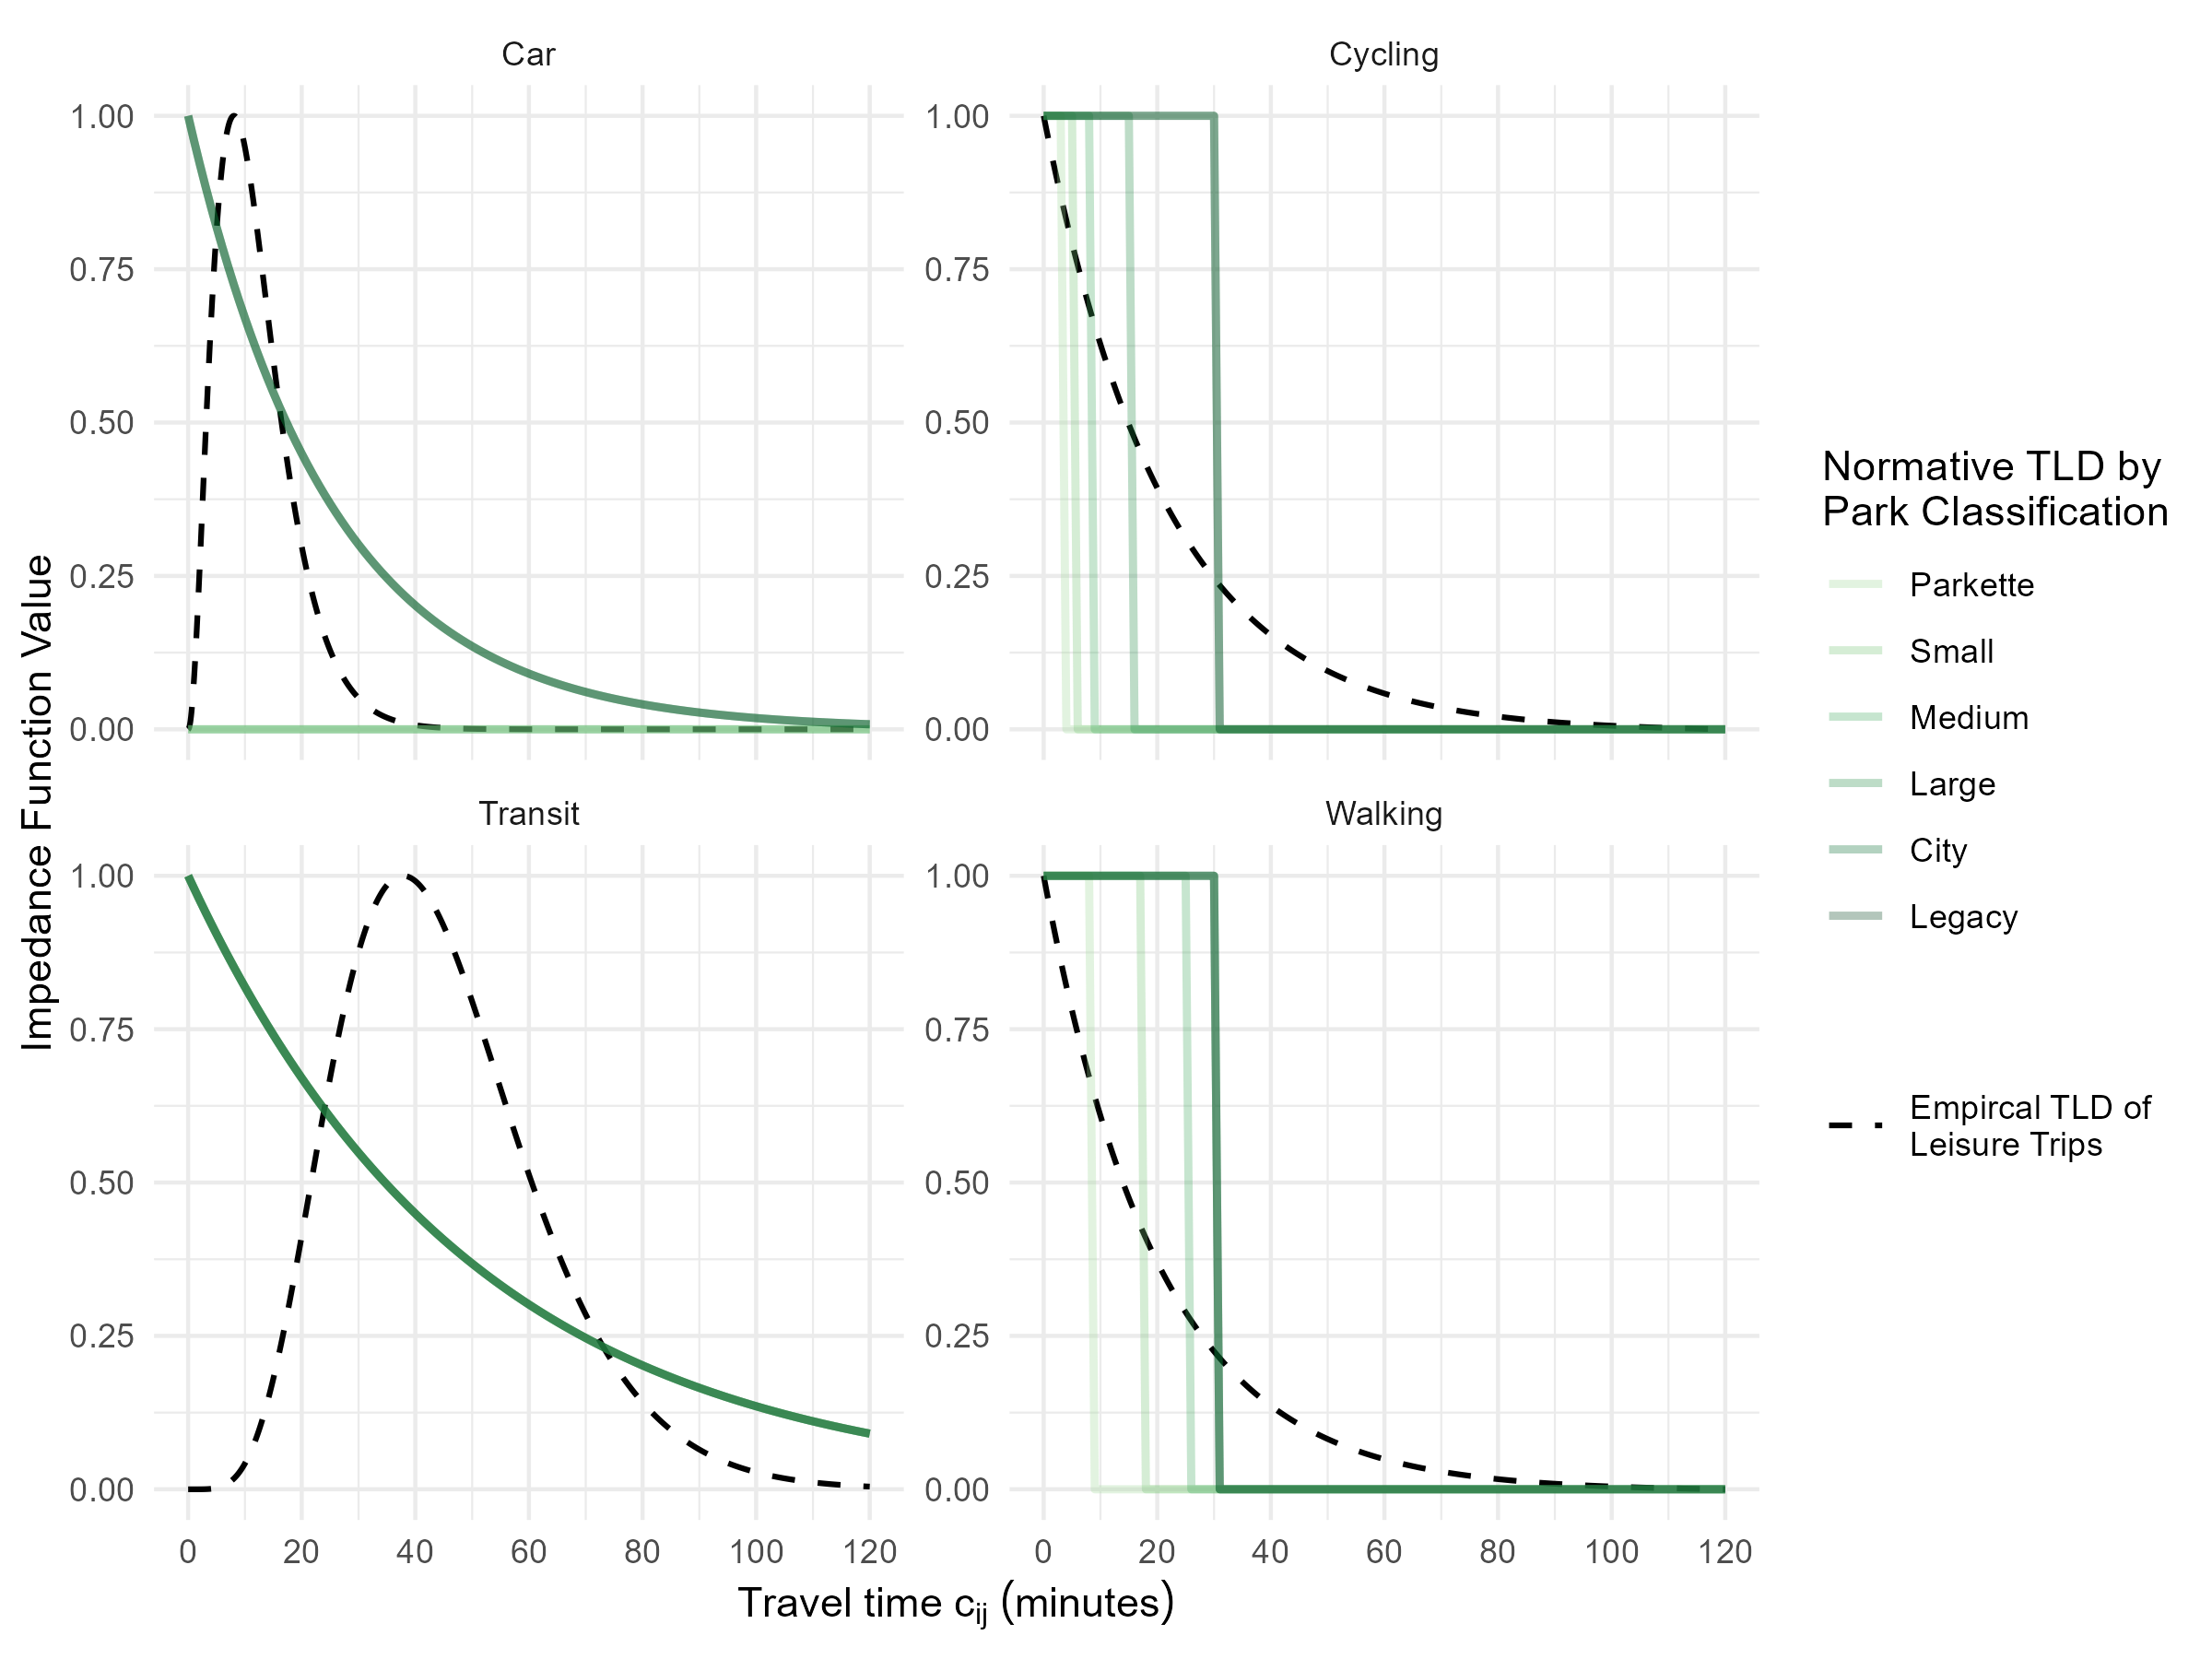
\includegraphics[width=6in]{./data/figures/chp2-norm_pos_impedance_mode_parktype_plot} 

}

\caption{\label{fig:chp2-norm_pos_impedance_mode_parktype_plot}  Scatter plot of cycle and walk travel times from origins to destinations by destination type for each park (either min mean travel time to park centroid, or to min mean travel time to park entrance). }\label{fig:unnamed-chunk-13}
\end{figure}

\subsection{Totally-constrained accessible parkland: all people demand it equally}\label{totally-constrained-accessible-parkland-all-people-demand-it-equally}

\subsubsection{A measure of parkland accessibility and population accessibility}\label{a-measure-of-parkland-accessibility-and-population-accessibility}

Totally-constrained accessibility \(V^T_{ij}\), a measure of parkland accessibility, is defined as follows:

\[
V^T_{ij} = K^T \cdot W_j^{(2)} \cdot f(c_{ij})
\] \{\#eq-total-constrained-access\}

Where:
- \(V^T_{ij}\) is the number of opportunities that can be accessed at origin zone \(i\) from destination zone \(j\),
- \(f(c_{ij})\) is the cost of travel \(c_{ij}\) from \(i\) to \(j\),
- the destination zone attraction mass \(W_j^{(2)}\) is the number of opportunities (i.e., the parkland in hectares at a park \(j\)), and
- \(K^T\) is the total constraint \(\frac{D}{\sum_i\sum_j W^{(2)}_jf(c_{ij})}\) that serves to proportionally allocate the opportunities \(D\) in the region and ensures units remain balanced.

Equation \ref{eq:total-constrained-access} represents totally-constrained access at \(i\) from \(j\), but it can be summarised as \(V^T_i\) by summing all \(V^T_{ij}\) for a specific \(i\) (i.e., \(V^T_i = \sum_j V^T_{ij}\)). \(V^T_i\) is linearly proportional to the Hansen-type accessibility measure \(S_i = W^{(2)}_jf(c_{ij})\). Furthermore, it is worth reiterating that the sum of \(V^T_{ij}\) across the region is equal to \(D\) i.e., \(\sum_i\sum_j V^T_{ij} = \sum_i V^T_{i} = D\).

A measure of population accessibility \(M^T_{ji}\) can also be defined using the totally-constrained formulation:
\[
M^T_{ji} = \hat K^T \cdot W_i^{(1)} f(c_{ji})
\] \{\#eq-total-constrained-market\}

Where:
- \(M^T_{ji}\) is the number of population that can be accessed from origin zone \(i\) by destination zone \(j\),
- \(f(c_{ji})\) is the cost of travel \(c_{ji}\) from \(j\) to \(i\),
- the destination zone attraction mass \(W_j^{(2)}\) is the number of opportunities (i.e., the parkland in hectares at a park \(j\)), and
- \(\hat K^T\) is the total constraint \(\frac{O}{\sum_i\sum_j W^{(2)}_jf(c_{ji})}\) that serves to proportionally allocate the population \(O\) in the region and ensures units remain balanced.

Equation \ref{eq:total-constrained-market} can also be summarised as \(M^T_j\) by summing all \(M^T_{ji}\) for a specific \(i\) (i.e., \(M^T_j = \sum_i M^T_{ji}\)). \(M^T_j\) is linearly proportional to the Hansen-type accessibility measure of market potential, hence, it is worth reiterating that the sum of \(M^T_{ji}\) across the region is equal to \(O\) i.e., \(\sum_i\sum_j M^T_{ji} = \sum_i M^T_{j} = O\).

\subsubsection{Multimodal extension}\label{multimodal-extension}

This measure can also be extended to reflect multiple modes. In this analysis, four modes are considered: the motorized car and transit options, and the non-motorized cycling and walking options. From origins to destinations, each mode has a different travel impedance function \(f^m(\cdot)\) and travel time cost \(c^m_{ij}\) (note: \(c^m_{ij}\) and \(c^m_{ji}\) are assumed to be equal). The totally-constrained formula is modified as follows include a sub-index \(m\):

\[
V^{mT}_{ij} = K^{mT} \cdot W_j^{(2)} \cdot f^m(c^m_{ij})
\]\{\#eq-total-constrained-multimodal-access\}

Where:
- \(V^{mT}_{ij}\) is the number of opportunities that can be accessed at origin zone \(i\) from destination zone \(j\) by mode \(m\),
- \(f^m(c^m_{ij})\) is the cost of travel \(c^m_{ij}\) by mode \(m\) from \(i\) to \(j\),
- the destination zone attraction mass \(W_j^{(2)}\) is the number of opportunities (i.e., the parkland in hectares at a park \(j\)), and
- \(K^{mT}\) is the modal total constraint \(\frac{D}{\sum_m\sum_i\sum_j W^{(2)}_jf^m(c^m_{ij})}\) that serves to proportionally allocate the opportunities \(D\) in the region and ensures units remain balanced.

Summarising equation \ref{eq:total-constrained-multimodal-access} as a measure of modal totally-constrained accessibility \(V^{mT}_i\) by summing all \(V^{mT}_{ij}\) for a specific \(i\) and \(m\) (i.e., \(V^{mT}_i = \sum_j V^{mT}_{ij}\)). \(V^{mT}_i\) can also be summed by mode to equal \(V^{T}_i\) (i.e., \(\sum_m V^{mT}_i = V^{T}_i\)) and summed across the region to equal \(D\) (i.e., \(\sum_m\sum_i\sum_j V^{mT}_{ij} = \sum_m\sum_i V^{mT}_{i} = D\)).

Transposing \(i\) and \(j\) and expressing \(M^{mT}_{ji}\), the multimodal `market potential' or the population accessible by mode can also be defined using the totally-constrained formulation, with similar parameters as previously defined.
\[
M^{mT}_{ji} = \hat K^{mT} \cdot W_i^{(1)} f^m(c^m_{ji})
\] \{\#eq-total-constrained-multimodal-market\}

\subsubsection{Multimodal and multi-opportunity type extension}\label{multimodal-and-multi-opportunity-type-extension}

And lastly, the measure can also be extended to reflect multiple opportunities types (sub-index \(y\)), in addition to multiple modes.

\[
V^{ymT}_{ij} = K^{mT} \cdot W_j^{y} \cdot f^m(c^m_{ij})
\]\{\#eq-total-constrained-multimodal-multiopp-access\}

If there was a multiple population groups considered, then a \(M^{ymT}_{ji}\) could be specified. But in this analysis, this data will not be incorporated. However, market potential per mode per park can be specified:

\[
M^{ymT}_{ji} = \hat K^{mT} \cdot W_i^{(1)} f^m(c^m_{ji})
\] \{\#eq-total-constrained-multimodal-multiopp-market\}

\subsubsection{Representing constrained accessibility as a ratio}\label{representing-constrained-accessibility-as-a-ratio}

parkland accessible per capita:
\[
v^{T}_{i} = V^{T}_{i} /P_{i}^{m}
\]\{\#eq-total-constrained-access-per-capita\}

\[
v^{mT}_{i} = V^{mT}_{i} /P_{i}^{m}
\]\{\#eq-total-constrained-multimodal-access-per-capita\}

\[
v^{ymT}_{i} = V^{ymT}_{i} /P_{i}^{ym}
\]\{\#eq-total-constrained-multimodal-multiopp-access-per-capita\}

Per population \(P_i\) per zone \(i\) overall or a subset, as in population of mode user \(m\) or population of mode user for a specific park classification \(y\).

This can likewise be applied to market potential, representing population accessible per parkland area:
\[
m^{T}_{j} = M^{T}_{j} /O_{j}^{m}
\]\{\#eq-total-constrajned-access-per-capjta\}

\[
m^{mT}_{j} = M^{mT}_{j} /O_{j}^{m}
\]\{\#eq-total-constrajned-multjmodal-access-per-capjta\}

Per parkland \(O_j\) per zone \(i\) overall or a subset, as in opportunities reached by mode \(m\) or opportunities reached by mode of a specific park classification \(y\).

\section{Results}\label{results}

The figure demonstrates the accessible to all parks for each DB (recall, out of the total 1607 parks), as an overview of the city.
{[}1 Toronto DB plot - featuring accessibility to all parks considering `average' modal impedance{]}

If interested in the coverage of the parks, the following figure demonstrates the accessibility to people for each DB, in the context of their travel to parks.
{[}1 Toronto DB plot - featuring accessibility to all people considering `average' modal impedance{]}

\subsection{Potential access to parks}\label{potential-access-to-parks}

Focusing on the accessible number of parks: the following plot demonstrates a disaggregated version of figure above. Each plot demonstrates the number of parks that are accessible, by mode. Again, the embedded assumption is the number of parkland in the city is allocated to each DB based on the travel impedance of that mode's zone relative to all the travel impedance of all modes in the region.
{[}4 Toronto DB plots - featuring accessibility to all parks by mode{]}

{[}4 Toronto DB plots, summarised by neighbourhood - featuring accessibility to ONLY large parks by mode{]}

{[}4 Toronto DB plots, summarised by neighbourhood - featuring accessibility to ONLY small parks by mode{]}

{[}4 Toronto DB plots - featuring accessibility to all parks per capita by mode{]}

{[}summary table of top 5, middle 5, and bottom 5 neighbourhoods{]}

\subsection{Potential access to peopulation}\label{potential-access-to-peopulation}

If interested in using totally-constrained accessibility as an indicator of service provision, conceptualing the `market pontential' variant is useful to yield values of `number of people that can access parks' for the zonal unit of question.

The following is the access to people, by mode. Notably, it is not correlated with opportunities, as there is a mis-match in population and parkland in certain neighbourhood (see fig..X)
{[}4 Toronto DB plots - featuring accessibility to all people by mode{]}

The following is the access to people, by mode:
{[}4 Toronto DB plots, summarised by neighbourhood - featuring accessibility to people from ONLY large parks by mode{]}

{[}4 Toronto DB plots, summarised by neighbourhood - featuring accessibility to people from ONLY small parks by mode{]}

{[}4 Toronto DB plots - featuring accessibility to all people per parkland capita by mode{]}

{[}summary table of top 5, middle 5, and bottom 5 neighbourhoods{]}

\section{Concluding remarks}\label{concluding-remarks}

\begin{itemize}
\tightlist
\item
\end{itemize}

\chapter{CHP 3 - Singly constrained spatial access to park space}\label{chp-3---singly-constrained-spatial-access-to-park-space}

THIS CHAPTER WILL \ldots{}

\chapter{CHP 4 - Multi-modal totally- and singly- constrained spatial access to park space}\label{chp-4---multi-modal-totally--and-singly--constrained-spatial-access-to-park-space}

THIS CHAPTER WILL \ldots{}

\chapter{CHP 5 - Comparing constrained and unconstrained access to park space}\label{chp-5---comparing-constrained-and-unconstrained-access-to-park-space}

THIS CHAPTER WILL \ldots{}

\chapter*{Conclusion}\label{conclusion}
\addcontentsline{toc}{chapter}{Conclusion}

Concluding\ldots{}

\begin{itemize}
\tightlist
\item
  open and reproducibility of methods learned are discussed (text from \emph{``TTS2016R: A data set to study population and employment patterns from the 2016 Transportation Tomorrow Survey in the Greater Golden Horseshoe area, Ontario, Canada''} is included)
\item
  how constrained measures can be interpreted,
\item
  how this interpretation can aid policy makers-- per capita, per any other zonal property. comparisions between regions, between times.
\item
  how policy makers can ultimately use this to plan for inequities (some text pulled from \emph{``Searching for fairness standards in the transportation literature''}).
\item
  Future research directions (?)
\end{itemize}

\chapter*{References}\label{references}
\addcontentsline{toc}{chapter}{References}

Placeholder

\phantomsection\label{refs}
\begin{CSLReferences}{1}{0}
\bibitem[\citeproctext]{ref-toronto_NEI_2014}
City of Toronto. (2014). TSNS 2020 neighbourhood equity index methodological documentation. City of Toronto - Social Policy Analysis; Research. Retrieved from \url{https://www.toronto.ca/wp-content/uploads/2017/11/97eb-TSNS-2020-NEI-equity-index-methodology-research-report-backgroundfile-67350.pdf}

\bibitem[\citeproctext]{ref-toronto_parkland2019}
City of Toronto. (2019). Parkland strategy: Growing toronto parkland. Toronto, Ontario: City of Toronto - Parks, Forestry; Recreation. Retrieved from \url{https://www.toronto.ca/wp-content/uploads/2019/11/97fb-parkland-strategy-full-report-final.pdf}

\bibitem[\citeproctext]{ref-toronto_neighbourhoods2024}
City of Toronto. (2024). Neighbourhoods (Version Oct 15, 2024). City of Toronto. Retrieved from \url{https://open.toronto.ca/dataset/neighbourhoods/}

\bibitem[\citeproctext]{ref-toronto_greenspaces2025}
City of Toronto. (2025). Green spaces in toronto (Version Apr 29, 2025). City of Toronto. Retrieved from \url{https://open.toronto.ca/dataset/green-spaces/}

\bibitem[\citeproctext]{ref-data_management_group_tts_2023}
Data Management Group. (2023). {TTS} - {Transportation} {Tomorrow} {Survey} 2023. Retrieved from \url{https://tts2023.ca/en/index.php}

\bibitem[\citeproctext]{ref-paezMeasuringAccessibilityPositive2012}
Páez, A., Scott, D. M., \& Morency, C. (2012). Measuring accessibility: Positive and normative implementations of various accessibility indicators. \emph{Journal of Transport Geography}, \emph{25}, 141--153. http://doi.org/\href{https://doi.org/10.1016/j.jtrangeo.2012.03.016}{10.1016/j.jtrangeo.2012.03.016}

\bibitem[\citeproctext]{ref-pereiraR5rRapidRealistic2021}
Pereira, R. H. M., Saraiva, M., Herszenhut, D., Braga, C. K. V., \& Conway, M. W. (2021). r5r: Rapid realistic routing on multimodal transport networks with r \(^{\textrm{5}}\) in r. \emph{Findings}. http://doi.org/\href{https://doi.org/10.32866/001c.21262}{10.32866/001c.21262}

\bibitem[\citeproctext]{ref-statcan_DAdef_2021}
Statistics Canada. (2021a). Dissemination area (DA) (Version 2023-07-07). Statistics Canada. Retrieved from \url{https://www12.statcan.gc.ca/census-recensement/2021/ref/dict/az/Definition-eng.cfm?ID=geo021}

\bibitem[\citeproctext]{ref-statcan_DBdef_2021}
Statistics Canada. (2021b). Dissemination area (DA) (Version 2023-07-07). Statistics Canada. Retrieved from \url{https://www12.statcan.gc.ca/census-recensement/2021/ref/dict/az/Definition-eng.cfm?ID=geo014}

\bibitem[\citeproctext]{ref-statcan_reppoint_2021}
Statistics Canada. (2021c). Representative point (Version November 17, 2021). Statistics Canada. Retrieved from \url{https://www12.statcan.gc.ca/census-recensement/2021/ref/dict/az/definition-eng.cfm?ID=geo040}

\end{CSLReferences}

\end{document}
